\documentclass{beamer}

\usepackage{beamerthemeCambridgeUS}
\usepackage{graphics}
\usepackage{graphicx}
\usepackage{hyperref}
\usepackage{StyleFiles/algorithm}
\usepackage{StyleFiles/algorithmic}
\usepackage{amssymb}
\usepackage{fancyhdr}
\usepackage{eucal}
\usepackage[T1]{fontenc}
\usepackage{lmodern}
\usepackage{amsthm}

\title[Player Behavior and Team Strategy]{Player Behavior and Team Strategy in Robocup Simulation 3D League}
\author[Georgios Methenitis]{Georgios Methenitis}
\institute[TUC]{Technical University of Crete}
\date[Chania, 2012]{Chania, August, 2012}
\subject{Computational Sciences}

\begin{document}

\newcommand{\putat}[3]{\begin{picture}(0,0)(0,0)\put(#1,#2){#3}\end{picture}}

  \frame
  {
    \titlepage
    \begin{center}
    \begin{small}
     Thesis Committee\\
    Assistant Professor Michail G. Lagoudakis (ECE)\\
Assistant Professor Georgios Chalkiadakis (ECE)\\
Professor Minos Garofalakis (ECE)\\
    \end{small}
    \end{center}
  }

  
  \frame
  {
    \frametitle{Abstract}
    This thesis presents a complete team design for the RoboCup 3D Simulation League focusing on player behavior, team strategy, and team coordination. Our agents are designed in a way that enables them to act effectively both autonomously and as members of the team.

  }  


  \frame
  {
    \frametitle{Outline of Topics}

    \tableofcontents
  }

 \section{Background}

 \subsection*{RoboCup}
  \frame
  {
    \frametitle{Robocup Competition}
    \begin{itemize}[<+->]
    	\item RoboCup is an international robotics competition.
        \item Founded in 1997.
        \item The official goal of the project is stated as an ambitious endeavor: ``By the year 2050, a team of fully autonomous humanoid robot soccer players shall win the soccer game, complying with the official rule of the FIFA, against the winner of the most recent World Cup''.
     \end{itemize}

  }
  
  \subsection*{RoboCup Leagues}
   
  \frame
  {
    \frametitle{Soccer}
    Standard Platform League
    \begin{itemize}
    	\item Same robot platform
     \end{itemize}
   	\begin{figure}[t!] 
\centering
    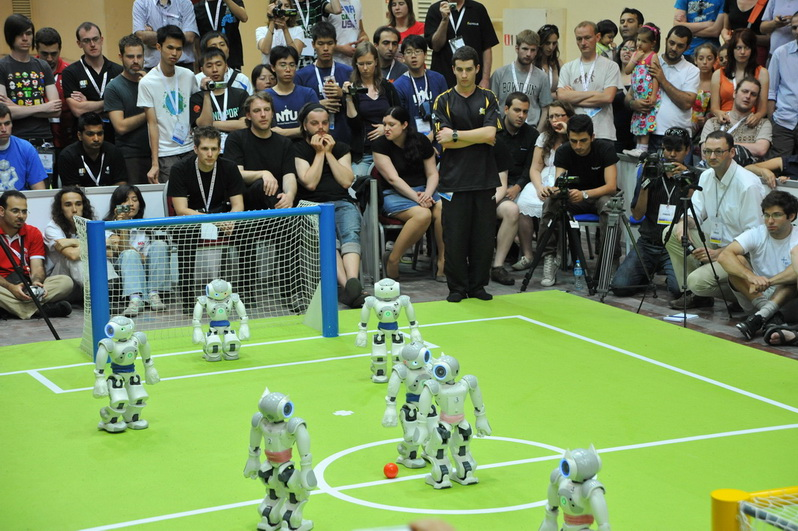
\includegraphics[width=0.6\textwidth]{Chapter1/figures/spl.jpg}
\end{figure}
   	

  }  
  
  \frame
  {
    \frametitle{Soccer}
    Humanoid League
   	\begin{figure}[t!] 
\centering
    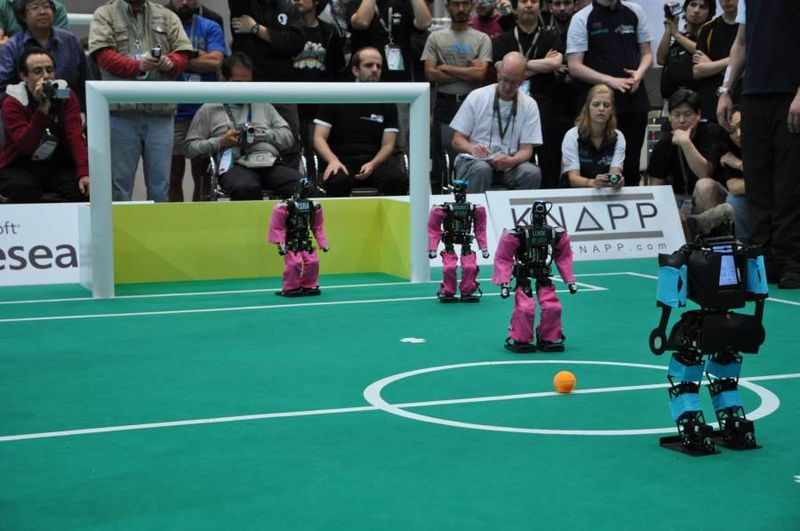
\includegraphics[height=3cm]{Chapter1/figures/kid2011.jpg}\ 
    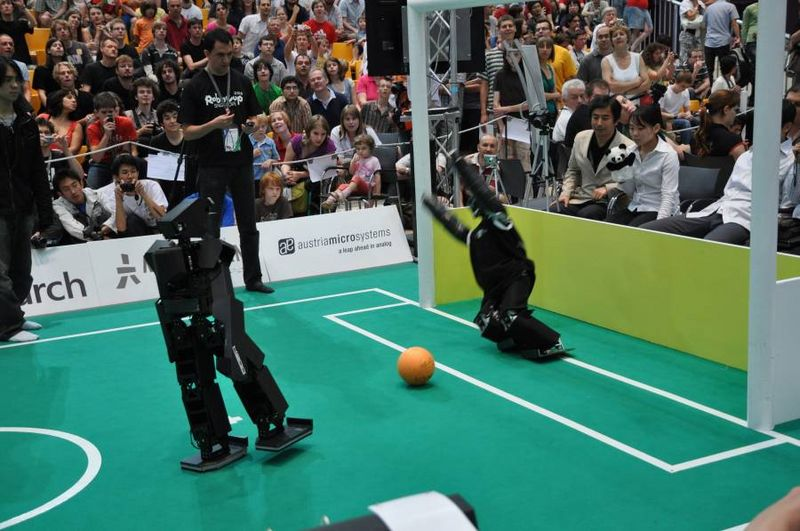
\includegraphics[height=3cm]{Chapter1/figures/teen2011.jpg}\ 
    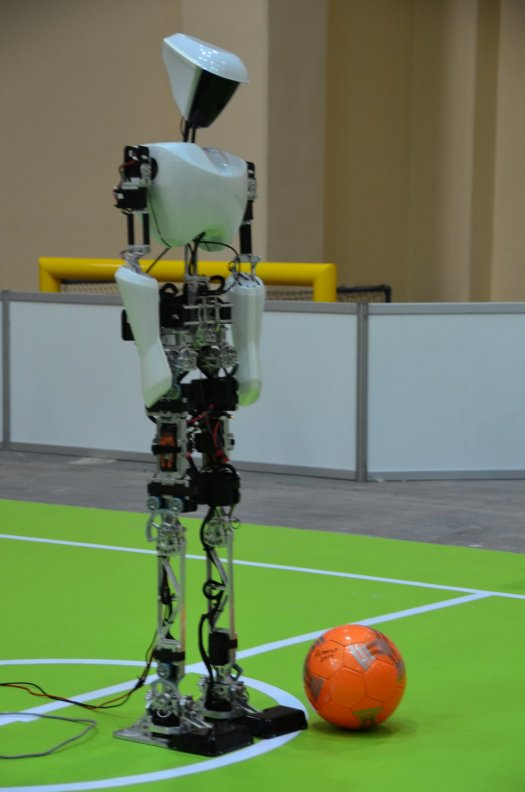
\includegraphics[height=3cm]{Chapter1/figures/adult2011.jpg}
\end{figure}
   	

  }
  
  \frame
  {
    \frametitle{Rescue}
\begin{figure}[t!]
\centering
  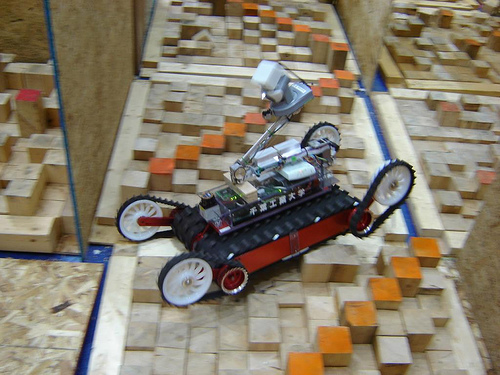
\includegraphics[width=0.6\textwidth]{Chapter1/figures/rescue.jpg}
\end{figure}
   	

  }
  
  
  \frame
  {
    \frametitle{@Home}
\begin{figure}[t!]
\centering
  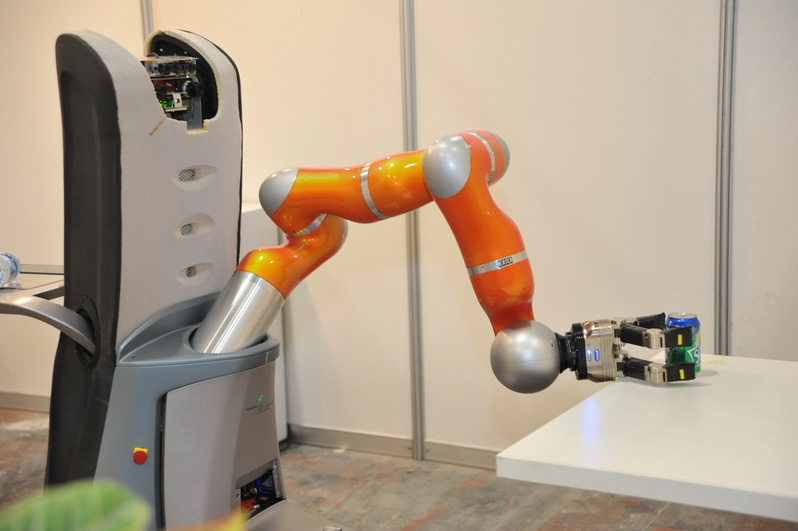
\includegraphics[width=0.6\textwidth]{Chapter1/figures/RoboCup@Home.jpg}
\end{figure}
   	

  }
  


  \subsection*{RoboCup Simulation League}
  \frame
  {
    \frametitle{Simulation League}
     \begin{itemize}[<+->]
    	\item One of the oldest leagues in RoboCup Soccer.
        \item Independently moving software players (agents).
        \item virtual field inside a computer.
        \item 2D League, 3D League.
     \end{itemize}
    

  }
  
  \frame
  {
    \frametitle{Simulation League 2D vs 3D}   
   	\begin{figure}[t!] 
\centering
    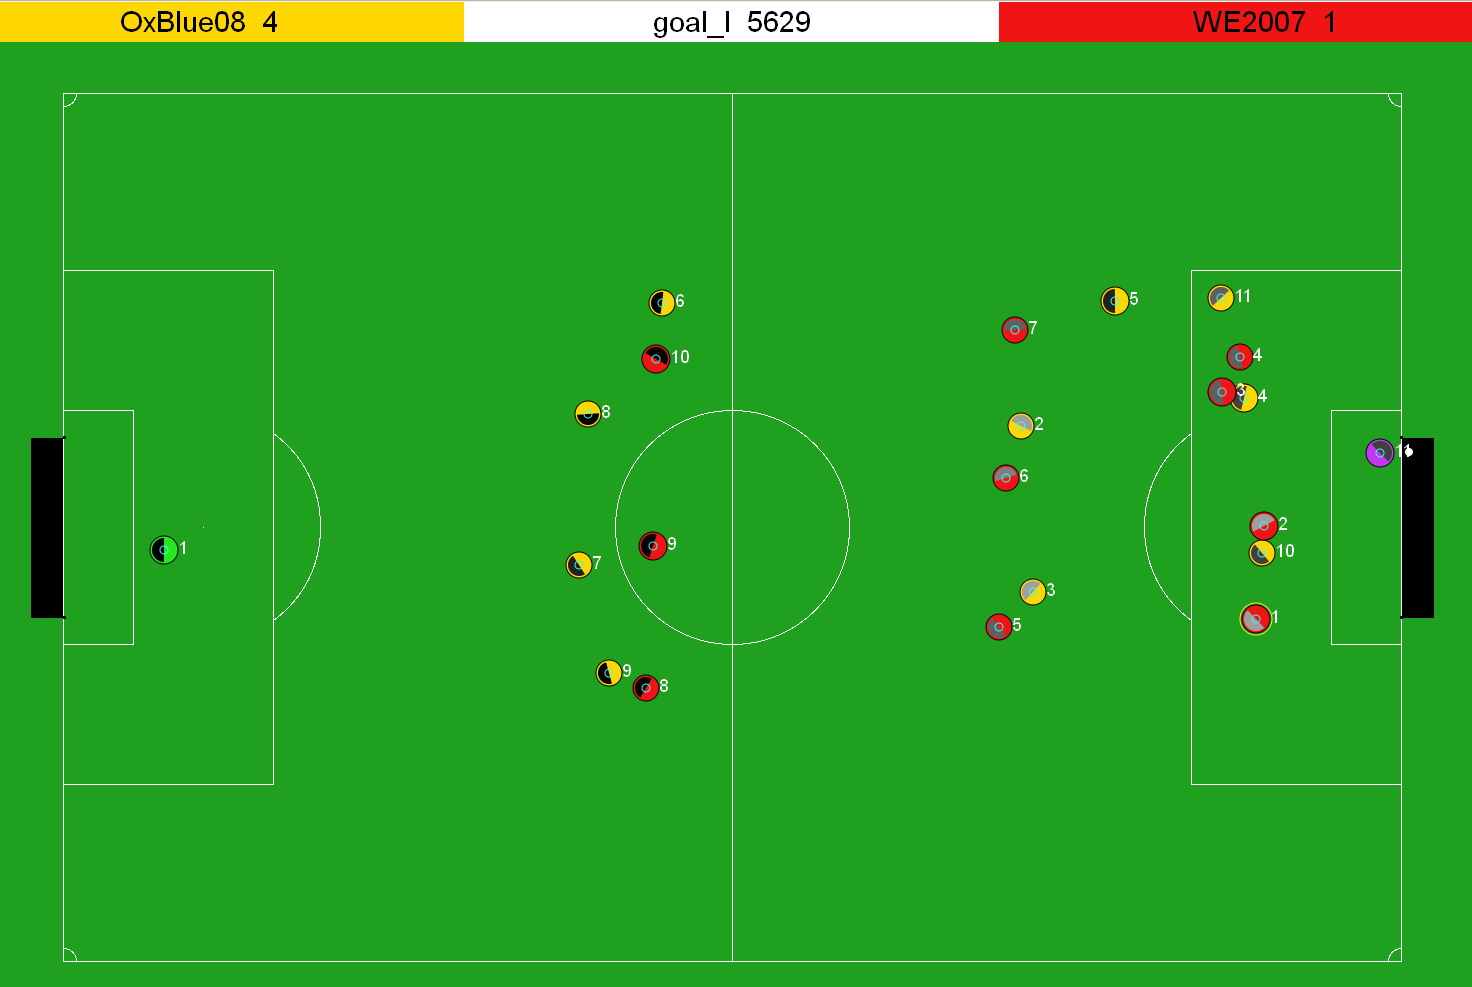
\includegraphics[height=3.5cm]{Chapter1/figures/2D.jpg}\	
    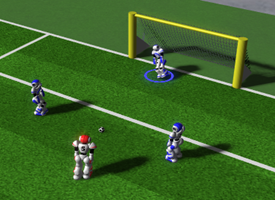
\includegraphics[height=3.5cm]{Chapter1/figures/3d.png}
\end{figure}
   	

  } 
  
  \subsection*{Simulation League 3D}
  \frame
  {
    \frametitle{3D Simulation Soccer}
    \begin{itemize}[<+->]
    \item At its beginning, spherical agent.
    \item In 2006, Fujitsu HOAP-2 robot.
    \item In 2008, Nao robot model.   
    \item \textbf{SimSpark} is used as the official Robocup 3D simulator.
    \end{itemize}
         
  }
  
  \frame
  {
    \frametitle{SimSpark}
    \begin{itemize}[<+->]
    \item \textbf{SimSpark} is a generic physics simulator system.
    \item Multiple agents in three-dimensional environment.
	\item \textit{Rcssserver3d} is the official competition environment for the RoboCup 3D Simulation League.

    \end{itemize}
         
  }
  
  \frame
  {
    \frametitle{Server's Versions}
    \begin{itemize}[<+->]
    \item Version 0.6.5
    \begin{description}
    \item[Players] 9
    \item[Length] 21m
    \item[Width] 14m
    \end{description}
    
    \item Version 0.6.6
     \begin{description}
    \item[Players] 11
    \item[Length] 30m
    \item[Width] 20m
    \end{description}
    \end{itemize}
         
  }
  
  \frame
  {
    \frametitle{Soccer Field}
    \begin{figure}[t!]
\centering
  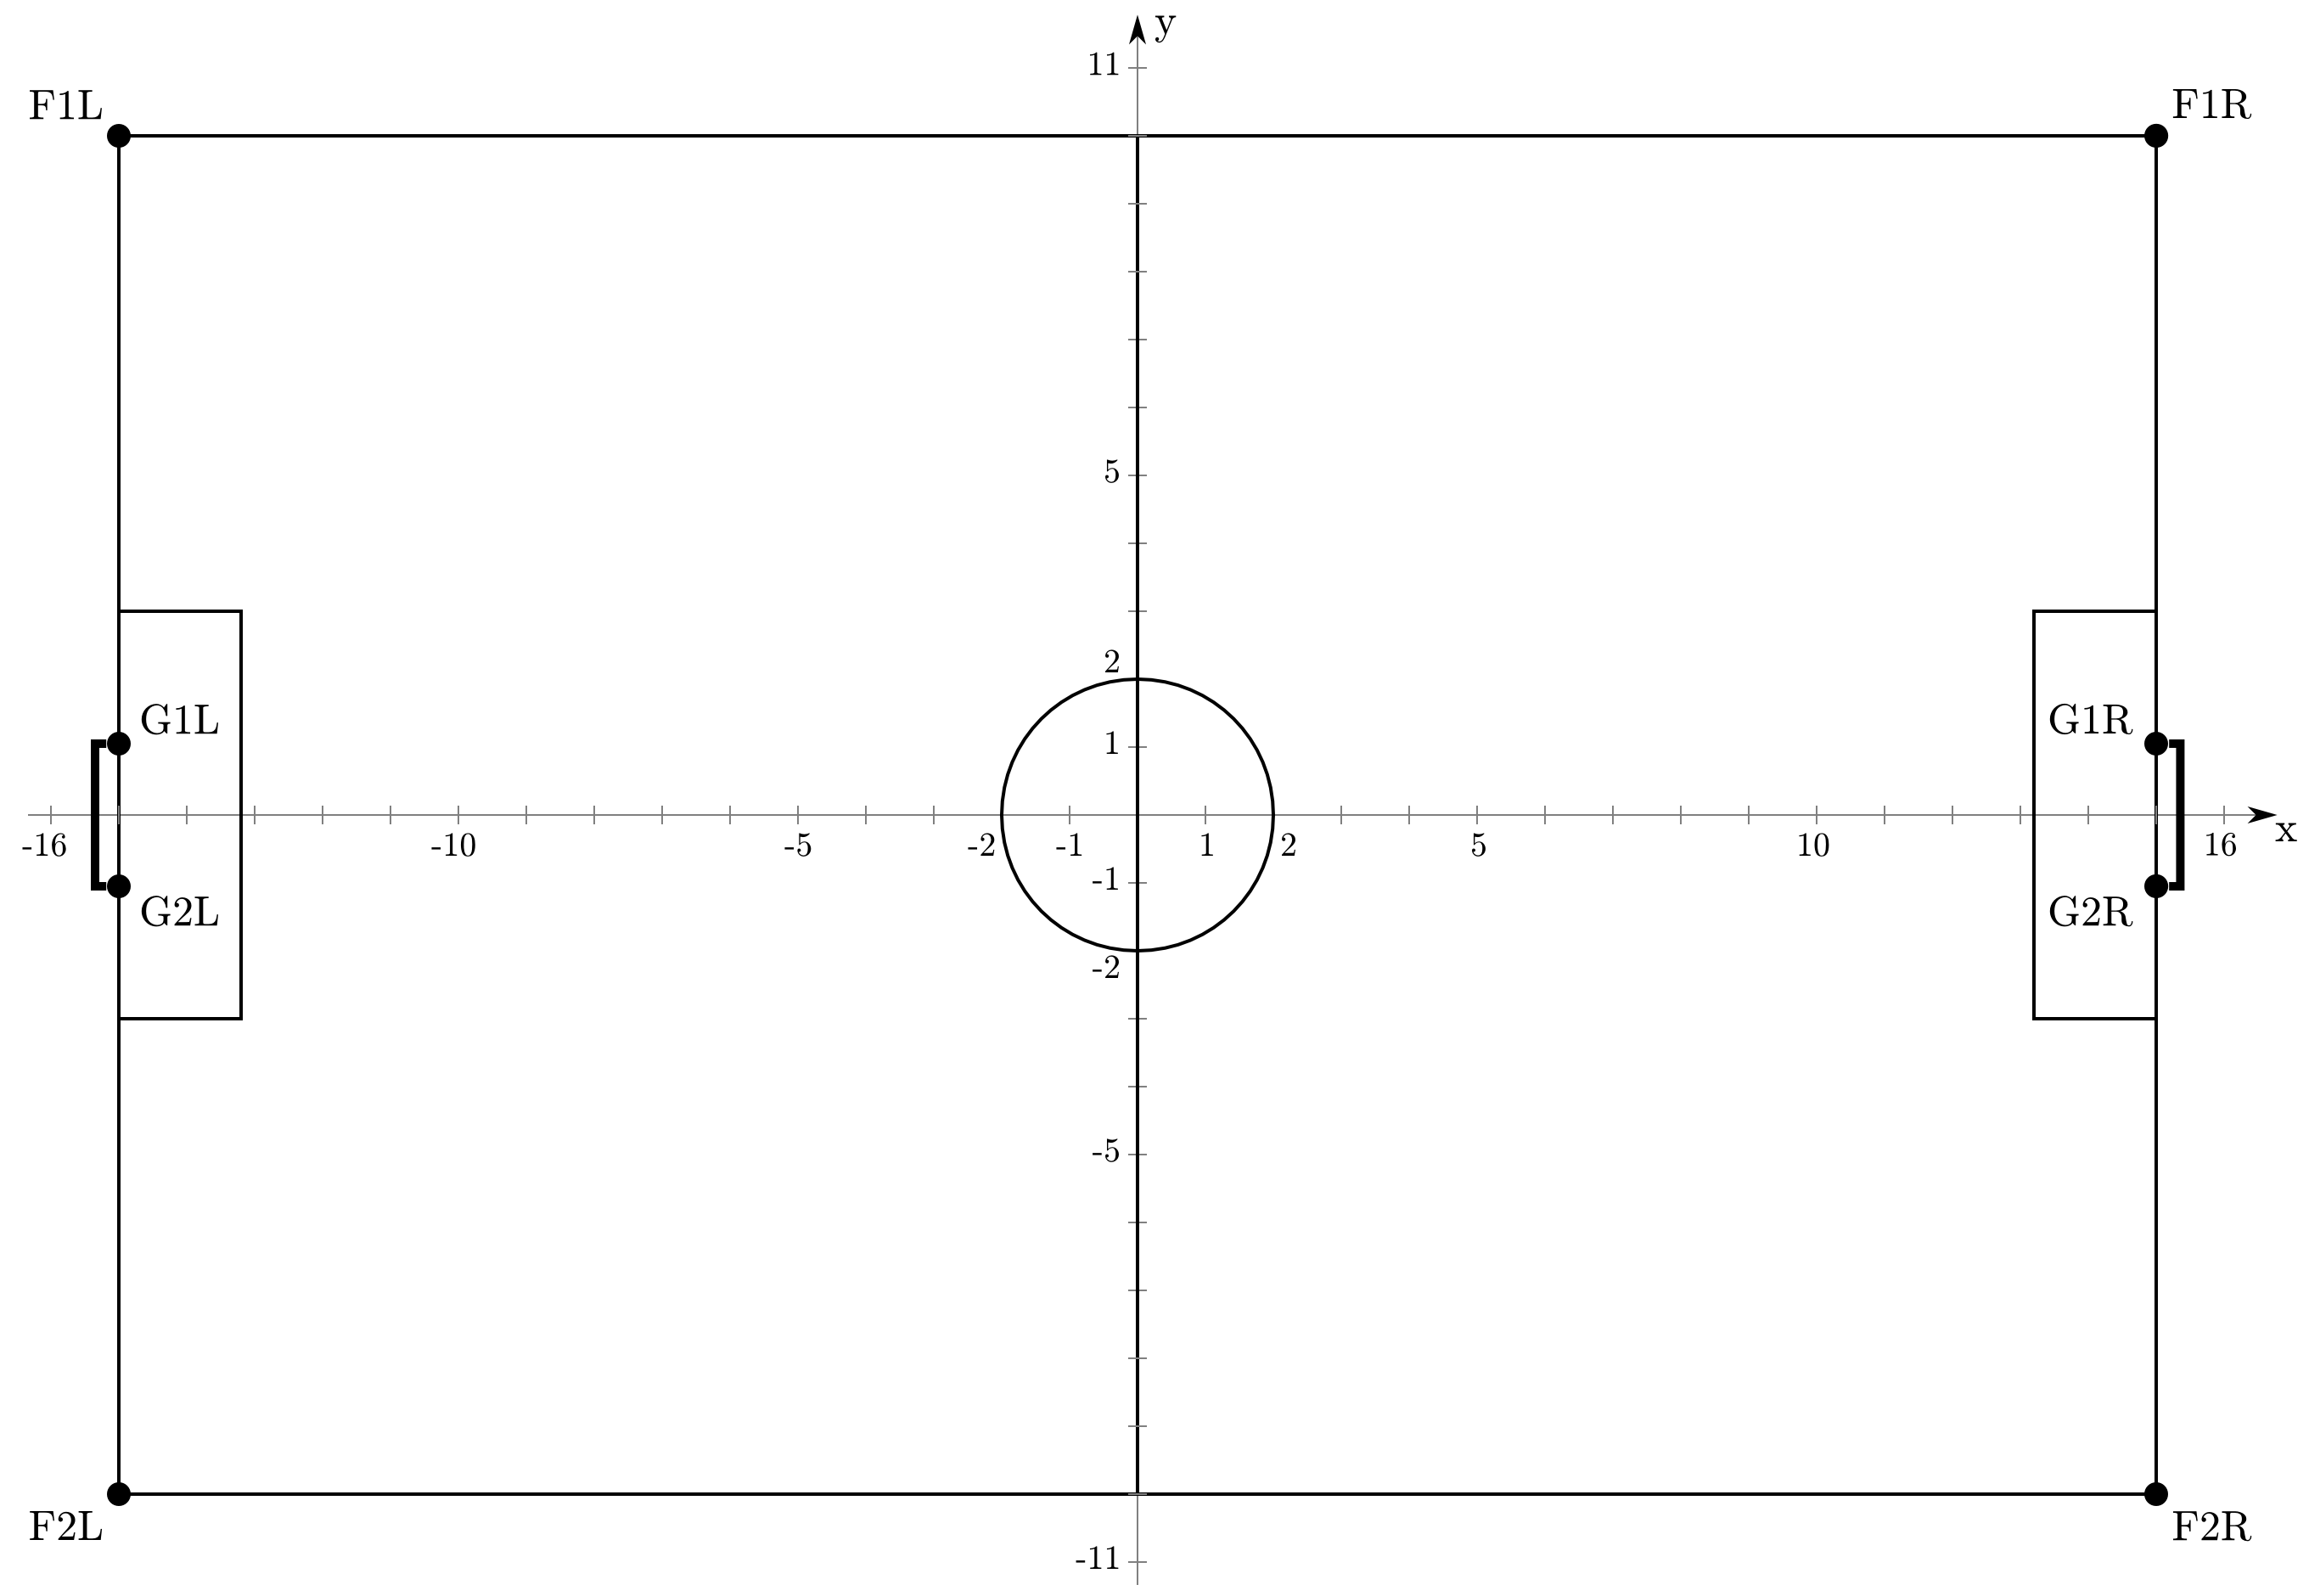
\includegraphics[width=0.8\textwidth]{Chapter2/figures/SoccerSimulation_FieldPlan.png}
\end{figure}
         
  }
  
  \frame
  {
    \frametitle{Robot Model}
    The Nao humanoid robot manufactured by Aldebaran Robotics. Its height is about 57cm and its 			weight is around 4.5kg. The simulated model comes with 22 degrees of freedom.
    \begin{figure}
\centering
  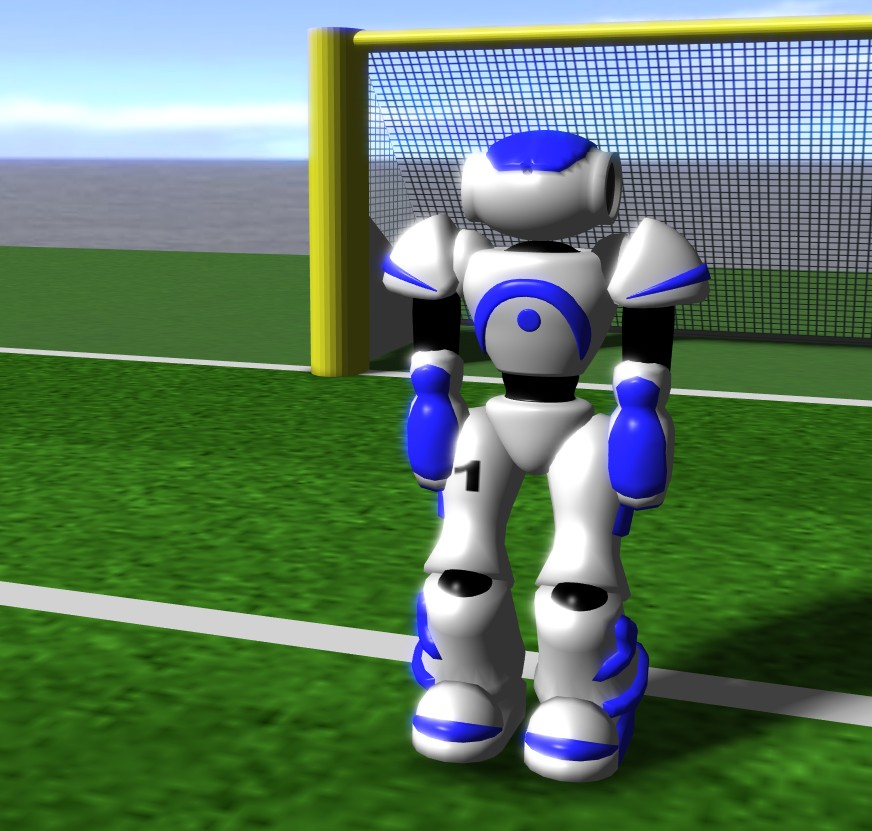
\includegraphics[trim=7cm 0cm 0cm 0cm, clip, width=0.4\textwidth]{Chapter2/figures/629px-Models-nao.jpg}
  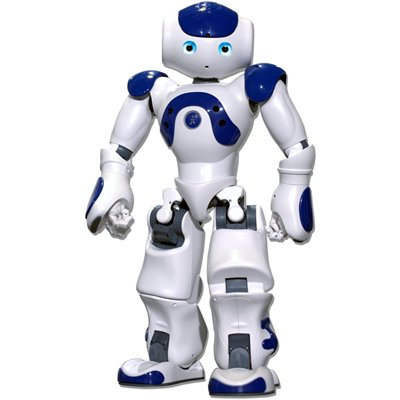
\includegraphics[width=0.4\textwidth]{Chapter2/figures/RealNao.jpg}
\end{figure}

   
  }
  
  \frame
  {
    \frametitle{Server}
    The SimSpark server hosts the process that manages and advances the simulation.
    \begin{itemize}[<+->]
	\item Simulation Cycle, 20ms
	\item Sense
	\item Think
	\item Act
    \end{itemize}
	\begin{figure}[t!]
	\centering
  		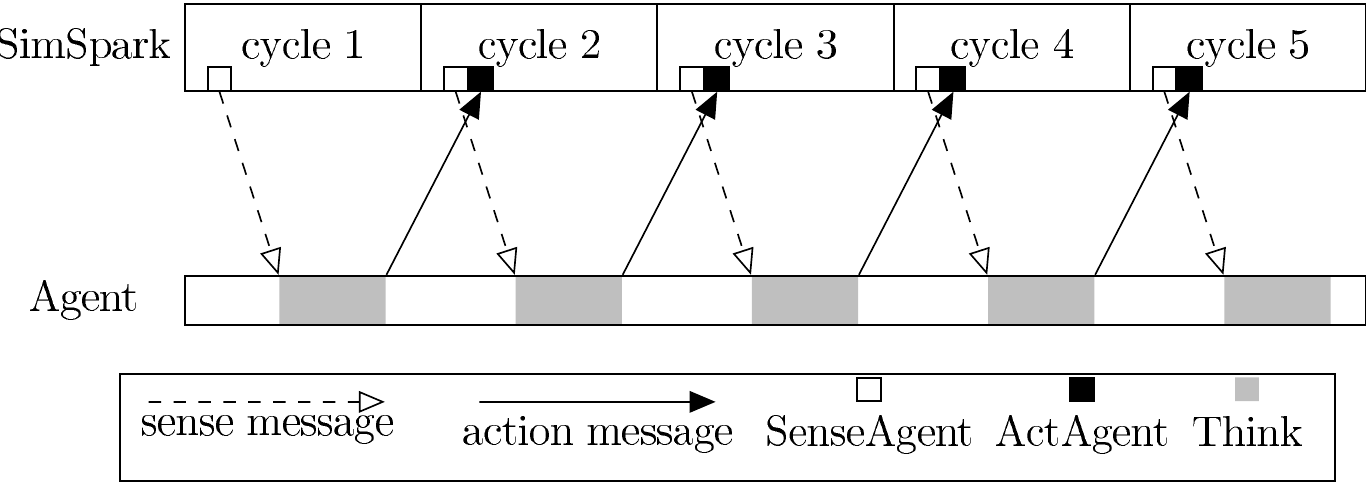
\includegraphics[width=0.6\textwidth]														{Chapter3/figures/SimulationUpdateLoopSynchronizationBetweenSimSparkAndAgent.png}
	\end{figure}
     
  }
  

  \begin{frame}
  \frametitle{Agent Perceptors}
Perceptors are the senses of an agent, allowing awareness of the agent's model state and the environment.  
  
    \begin{itemize}[<+->]
    \item HingeJoint Perceptor

    \item ForceResistance Perceptor

    \item GyroRate Perceptor

    \item Accelerometer Perceptor

    \item Vision Perceptor

    \item Hear Perceptor

    \item GameState Perceptor

    \end{itemize}
  \end{frame}
  
  \begin{frame}
    
    \frametitle{Agent Effectors}
    Effectors allow agents to perform actions within the simulation. Agents control them by sending messages to the server and the server changes the game state accordingly.

    \begin{itemize}[<+->]
     
    \item Create Effector

    \item HingeJoint Effector

    \item Synchronize Effector

    \item Init Effector

    \item Beam Effector

    \item Say Effector

    \end{itemize}
       
     
  \end{frame}
  
 \section{Player Skills}

  \subsection*{Architecture}

 \frame
  {
    \frametitle{Agents Architecture}
    
    \begin{figure}
	\centering
 	 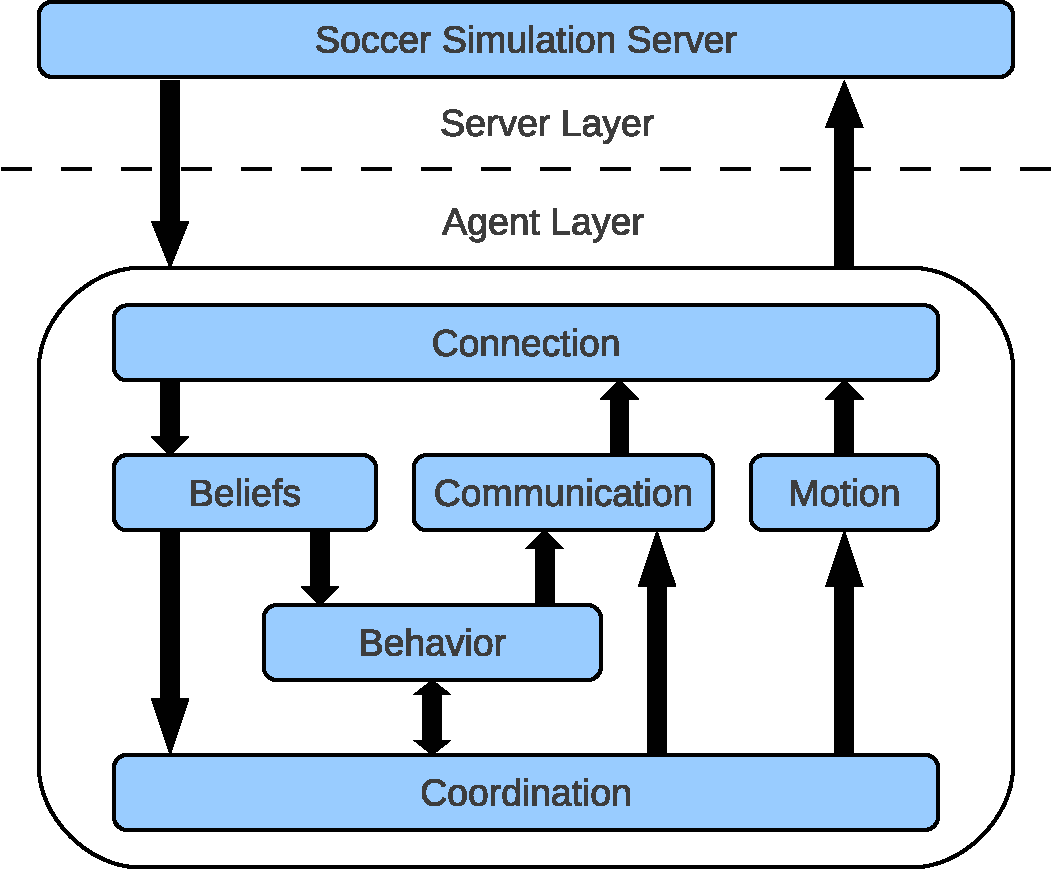
\includegraphics[width=0.7\textwidth]{Chapter3/figures/Arch.pdf}
	\end{figure}
    
  }
	


 \subsection*{General Skills}
  \frame
  {
    \frametitle{Connection}
    
	\begin{itemize}[<+->]
    \item Agent connected to the server at all times during a simulated game.
    \item Sense messages from the server every 20ms.
    \item Action messages, at the end of their think cycles.

    \end{itemize}

    
  }
  
  \frame
  {
    \frametitle{Perception}
    \begin{itemize}[<+->]
	\item Different from real robot soccer games.
    \item No raw data.
    \item Perceptor Messages.
    \item Agents update their beliefs and store sensors' data parsing these messages.
 	\end{itemize}
  
  }
  
  \begin{frame}[fragile]
  \frametitle{Perception Message Example}
  \begin{footnotesize}
  \begin{verbatim}(time (now 46.20))(GS (t 0.00) (pm BeforeKickOff))(GYR (n torso)
(rt 0.00 0.00 0.00))(ACC (n torso) (a 0.00 -0.00 9.81))(HJ (n hj
1)(ax 0.00))(HJ (n hj2) (ax 0.01))(See (G2R (pol 14.83 -11.81 1.
08))(G1R (pol 14.54 -3.66 1.12)) (F1R (pol 15.36 19.12 -1.91))(F
2R (pol 17.07 -31.86 -1.83)) (B (pol 4.51 -26.40 -6.15)) (P (tea
m AST_3D)(id 8)(rlowerarm (pol 0.18 -35.78 -21.65)) (llowerarm (
pol 0.19 34.94-21.49)))(L (pol 8.01 -60.03 -3.87) (pol 6.42 51.1
90 -39.13 -5.17))(L (pol 5.91 -39.06 -5.11) (pol 6.28-29.26 -4.8
8)) (L (pol 6.28 29.34 -4.95)(pol 6.16 -19.05 -5.00)))(HJ(n raj1
) (ax -0.01))(HJ (n raj2) (ax -0.00))(HJ (n raj3)(ax -0.00))(HJ(
n raj4) (ax 0.00))(HJ (n laj1) (ax 0.01))(HJ (n laj2) (ax 0.00)) ...
  \end{verbatim}
  \end{footnotesize}
\end{frame}


  \subsection*{Localization}
  \frame
  {
    \frametitle{Self-Localization}
    
	\begin{itemize}[<+->]
	\item Executed every three cycles (60ms).
    \item Localization uses the eight visible landmarks into the field.
    \begin{itemize}
    \item G1R, G2R, G1L, G2L
    \item F1R, F2R, F1L, F2L
    \end{itemize}
    \item Limited field of view (120 Degrees).

 	\end{itemize}

  }
  

  \frame
  {
    \frametitle{Simulated Nao's Restricted Field of View}

   \begin{figure}
	\centering
  	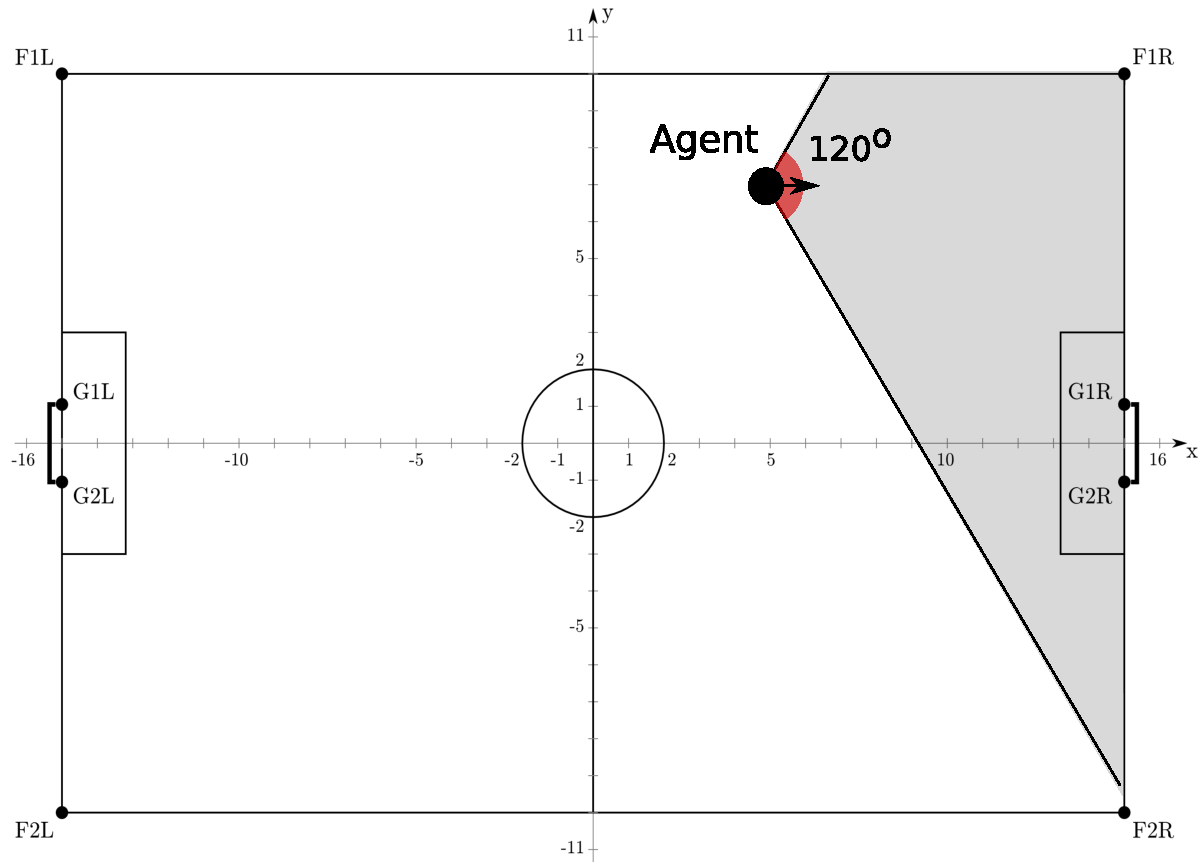
\includegraphics[width=0.8\textwidth]{Chapter3/figures/LViewAngle.pdf} 		
	\end{figure}
    
  }
    
  
  \frame
  {
    \frametitle{Self-Localization Technique}
	\begin{figure}
	\centering
  	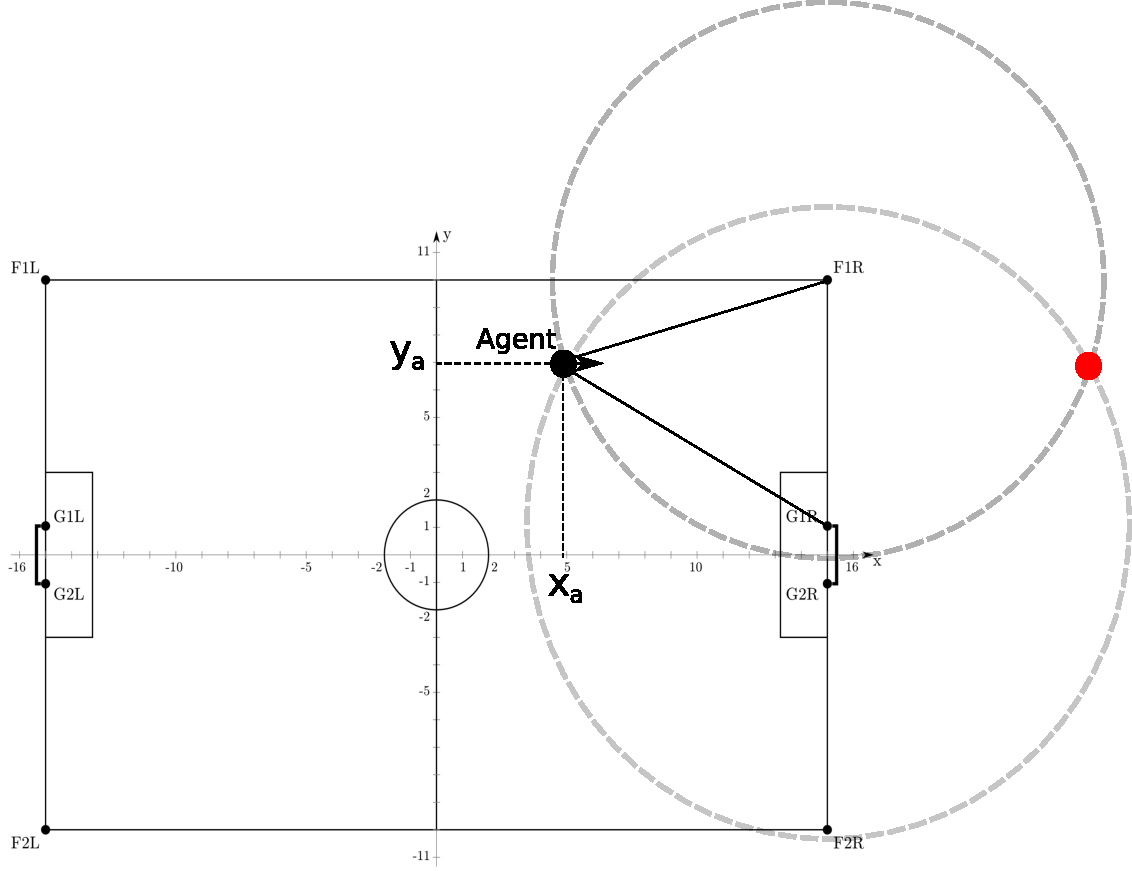
\includegraphics[width=0.8\textwidth]{Chapter3/figures/Localization.pdf}
	\end{figure}
   
    
  }
  
  \frame
  {
    \frametitle{Localization Results}
	\begin{figure}[t!]
\centering
  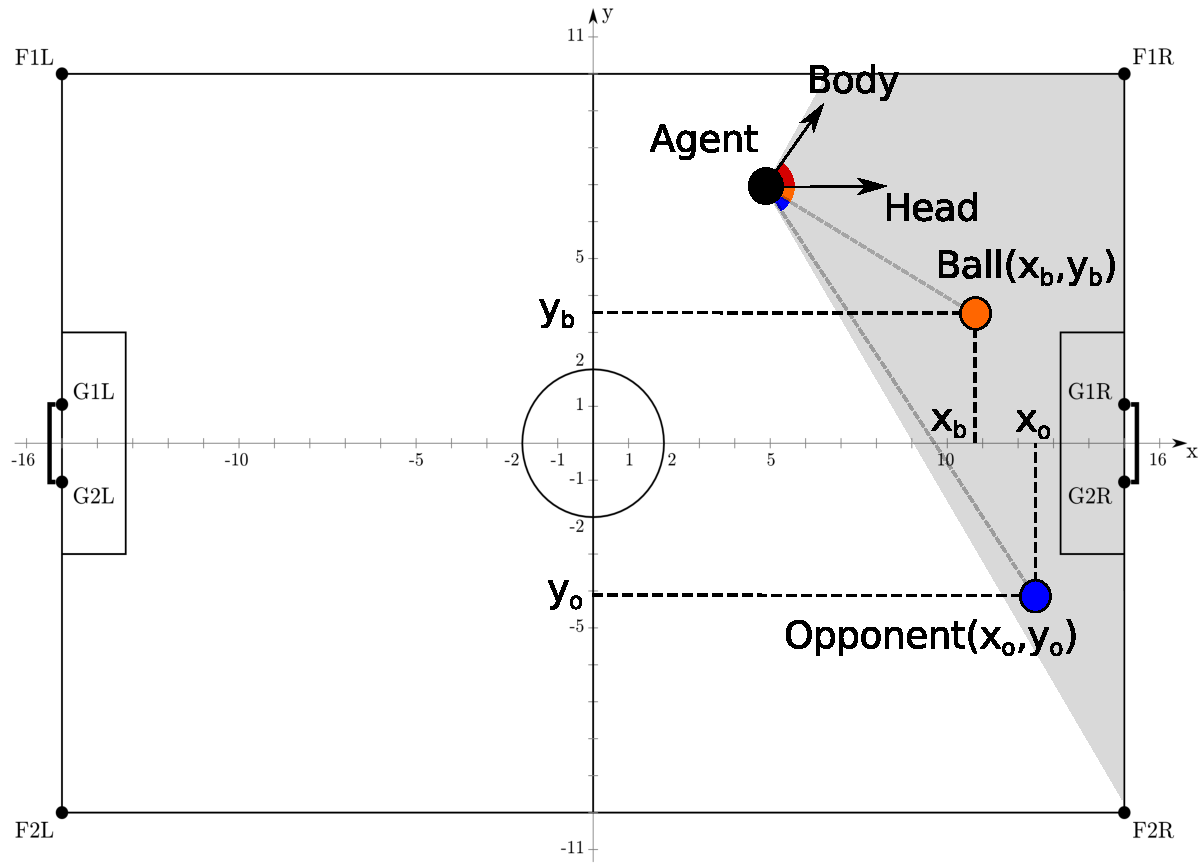
\includegraphics[width=0.8\textwidth]{Chapter3/figures/LocalizationResults.pdf}
 
\end{figure}
   
    
  }
  
  \frame
  {
    \frametitle{Localization Filtering}
	\begin{itemize}
	\item Absence of a more sophisticated probabilistic localization scheme.
	\pause
	\item Temporary absences of landmarks.
	\pause
	\item Noisy observations.
	\end{itemize}
   
    
  }
 
  \frame
  {
    \frametitle{Localization Filtering Algorithm}
\begin{algorithm}[H]
\caption{Localization Filtering}
\label{LocalizationFiltering}
\begin{algorithmic}[1]
\begin{footnotesize}
\STATE {\bf Input: }$LastEstimate$
\STATE {\bf Output: }$FilteredLocation$
\STATE $Queue$: a FIFO queue storing the $MaxSize$ (default=10) most recent estimates
\STATE 
\IF{$size(Queue) = 0$}
\STATE $Queue.Add(LastEstimate)$
\ELSIF{$LastEstimate \not\approx AverageLocation(Queue)$}
\STATE $Queue.Remove()$
\ELSE 
\IF{$size(Queue) = MaxSize$}
\STATE $Queue.Remove()$
\ENDIF
\STATE $Queue.Add(LastEstimate)$
\ENDIF
\RETURN $AverageLocation(Queue)$
\end{footnotesize}
\end{algorithmic}
\end{algorithm}
   
    
  }
  
  
  \subsection*{Motions and Movement}
  
  
  \frame
  {
    \frametitle{Nao's Anatomy}
    The simulated Nao robot comes with 22 degrees of freedom, corresponding to 22 hinge
joints. Figure 4.6 shows Nao�s anatomy with all joints, split in five kinematic chains
(head, left arm, right arm, left leg, right leg).
\begin{figure}
\centering
  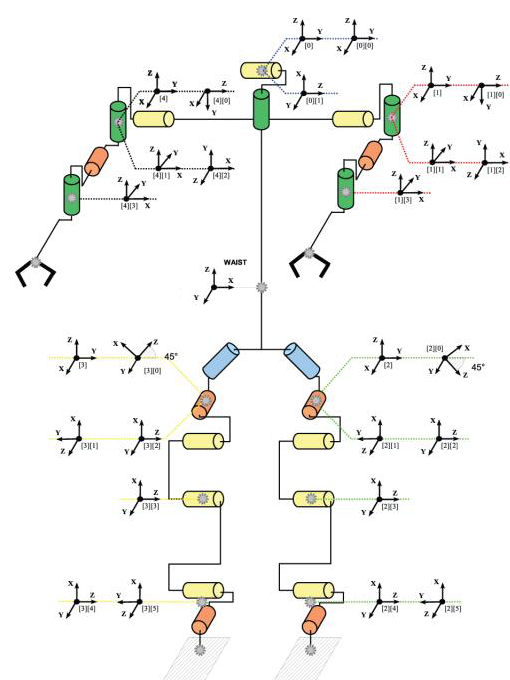
\includegraphics[width=0.3\textwidth]{figures/Models_NaoAnatomy.png}
\end{figure}

  }
  
  \frame
  {
    \frametitle{Motion and Movement}
    In robotics, a complex motion is commonly defined as a sequence of timed joint poses. A pose is a set of values for every joint in the robot's body or in a specific kinematic chain at a given time. 
For any given set of $n$ joints a pose at time $t$ is defined as:
\[
Pose(t)= \lbrace J_{1}(t), J_{2}(t), \ldots ,J_{n}(t) \rbrace
\]

  }
  
  \begin{frame}[fragile]
  \frametitle{XML-Based Motion Files}
  \begin{tiny}
  \begin{verbatim}<phase name="Start" next="Phase1">
   <effectors>
      Joint Values
   </effectors>
   <duration>duration</duration>
</phase>

<phase name="Phase1" next="Phase2">
   <effectors>
      Joint Values
   </effectors>
   <duration>duration</duration>
</phase>

<phase name="Phase2" next="Phase1">
   <effectors>
      Joint Values
   </effectors>
   <duration>duration</duration>
   <finalize>Final</finalize>
</phase>

<phase name="Final">
   <effectors>
      Joint Values
   </effectors>
   <duration>duration</duration>
</phase>
  \end{verbatim}
  \end{tiny}
  
  \putat{200}{30}{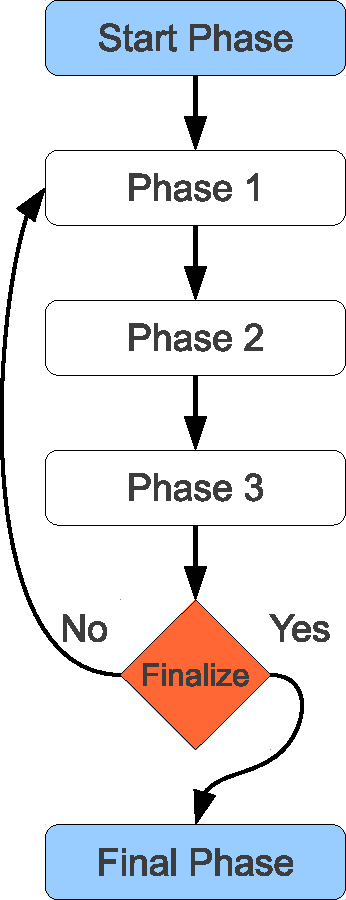
\includegraphics[width=0.2\textwidth]{figures/MotionSequence.pdf}}
  
\end{frame}


\frame
  {
    \frametitle{XML-Based Motion Controller}
    To generate motions for our agent we need to create a motion string, which encloses information about each joint's velocity. This velocity is computed as follows:
\[
Joint Velocity = \cfrac{Desired Joint Value - Current Joint Value}{PhaseDuration}
\]
A velocity value is calculated for each joint involved in the motion and the final output of the motion controller is sent to the server. In addition, zero velocity is set for every joint not included in the \texttt{effector} field of each phase, so that they stop moving. 

  }
  
  
   
 \begin{frame}[fragile]
  \frametitle{Text-Based Motion Files}
  \begin{footnotesize}
  \begin{verbatim}#WEBOTS_MOTION,V1.0
LHipYawPitch,LHipRoll,LHipPitch,LKneePitch,LAnklePitch,...
00:00:000,Pose1,0,-0.012,-0.525,1.05,-0.525,0.012,0,...
00:00:040,Pose2,0,-0.011,-0.525,1.05,-0.525,0.011,0,...
00:00:080,Pose3,0,-0.009,-0.525,1.05,-0.525,0.009,0,...
00:00:120,Pose4,0,-0.007,-0.525,1.05,-0.525,0.007,0,...
00:00:160,Pose5,0,-0.004,-0.525,1.05,-0.525,0.004,0,...
00:00:200,Pose6,0,0.001,-0.525,1.051,-0.525,-0.001,0,...
00:00:240,Pose7,0,0.006,-0.525,1.05,-0.525,-0.006,0,...
00:00:280,Pose8,0,0.012,-0.525,1.05,-0.525,-0.012,0,...
00:00:320,Pose9,0,0.024,-0.525,1.05,-0.525,-0.024,0,...
\end{verbatim}
  \end{footnotesize}
\end{frame}

\frame
  {
    \frametitle{Text-Based Motion Controller}
    The motion controller could be customized easily to perform these motions in different ways. The following parameters can be modified:
\begin{description}
	\item[Duration] The time between poses in simulation cycles. By default, $Duration=2$.
	\item[PoseStep] The step for advancing from pose to pose. By default, $PoseStep=1$, but we can subsample the motion with other values, e.g. for $PoseStep=2$, we execute pose1, pose3, pose5, ...
\end{description}
The desired velocity of each joint is computed by:
\[
JointVelocity = \cfrac {Desired Joint Value - Current Joint Value} {Duration \times CycleDuration}
\]
A velocity value is calculated for each joint involved in the motion and the final output of the motion controller is sent to the server. 

  }
  
  
\frame
  {
    \frametitle{Dynamic Motion Elements}
    \begin{description}
    \item[Walk Leaning] The XML-based walk motion can be dynamically modified to lean to
the right or to the left. This is accomplished by altering the joint values of the (left
or right) HipPitch and AnkePitch joints in specific phases of the walk motion.

    \item[Walk Slowdown] Increasing the phase durations dynamically by about 35\% yields a smooth approach to a stopping position.

    \item[Dynamic Turn] The text-based turn motion can be dynamically modified using a gain value
for scaling the resulting velocities in order to perform the motion in a smoother or
rougher way. By dynamically changing this value between 0.3 and 1.0, the agent is able to turn its body anywhere between 3 and 40 degrees.

    \end{description}

  }
  
  \frame
  {
	\begin{description}
	\item[X-Axis] Gain factor
	\item[Y-Axis] Agent turn
\end{description}	    
    
    \frametitle{Dynamic Turn Example}
    \begin{figure}
	\centering
 	 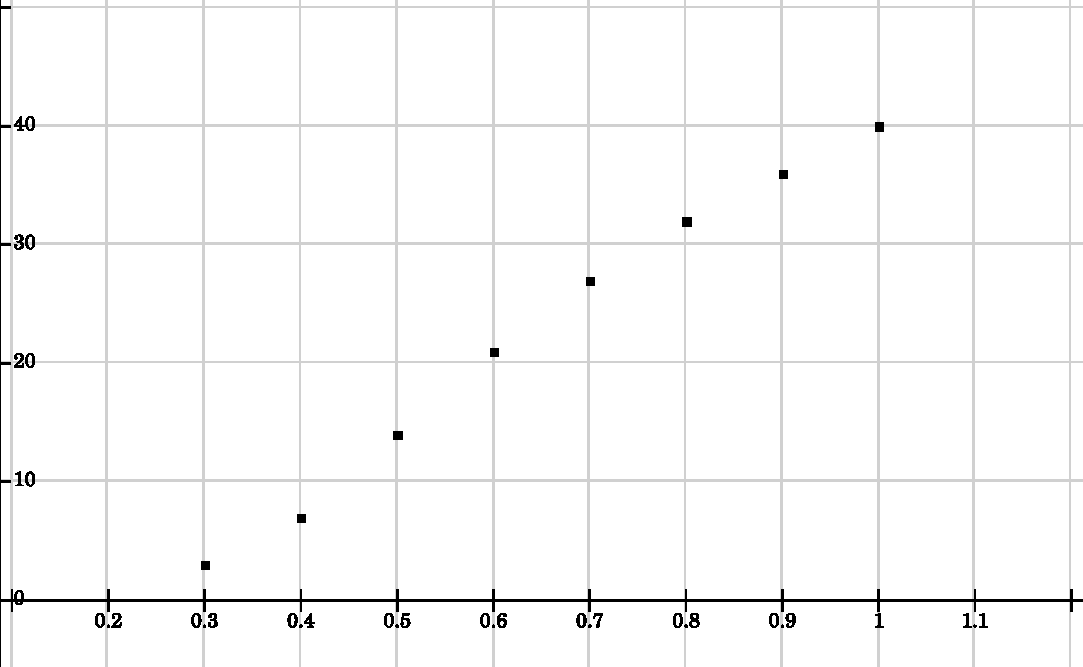
\includegraphics[width=0.8\textwidth]{figures/DynamicTurn.pdf}
	\end{figure}
  }
  
  
  \subsection*{Actions}
  \begin{frame}

    \frametitle{Actions}
    Actions are split into groups in terms of their complexity:
    \begin{description}
    \item[Basic Actions] Basic actions combine perceptual information and motion files in simple ways to achieve something useful.
    \item[Complex Actions] Complex actions combine perceptual information, motion files, and basic actions. They have a more complicated structure and aim to achieve specific goals.
    \end{description}
  
  \end{frame}
  
  \begin{frame}[allowframebreaks]
    \frametitle{Simple Actions}
	\begin{description}
    \item[Look Straight] Straight Moves the head to its nominal position. Both head joints are set to $0$.
    \item[Scan] Moves the head to perform periodic panning and tilting. 
    \item[Pan Head] Moves the head to perform periodic panning at zero tilt.
    \item[Track Object] Moves the head to bring a particular object to the center of the field of view. This action is applicable only when the object being tracked is visible, but is limited by the joint ranges. 
    \item[Track Moving Object] This action estimates the direction and the speed of a moving object using a small number of observations, obtained while performing the Track Object action. It records a set of five consecutive observations and another set of five consecutive observations delayed by a fixed time period (the default is 5 cycles).  The difference between the average positions of each set gives a vector that reveals the direction of motion. Taking the ratio of the magnitude of this vector and the time delay yields the speed of the moving object.
    \item[Find Opponent�s Goals] This action estimates the direction of the opponent's goal with respect to the agent by performing the Scan action.
	\item[Look For Ball] Turns the body of the agent, while performing the Scan action, until the ball appears within the field of view.
	\item[Turn To Ball] Turns the body of the agent towards the direction of the ball, while performing the Track Ball action. It can applied only when a ball is visible.
	\item[Turn To Localize] Turns the body of the agent, while performing the Pan Head action, until the agent's belief about its own location is updated with confidence.
	\item[Stand Up] Makes the agent stand up on its feet, after a confirmed fall on the ground, whether face-up or face-down. This action monitors the inertial sensors (accelerometers and gyroscopes) to check if our agent has fallen on the ground. Incoming gyroscope and accelerometer values above a specific threshold indicate a possible fall, but this has to be confirmed, because it is not unusual to receive values above threshold due to collisions without a fall. To confirm a fall, the action checks the force resistance perceptors located under the agent's feet. If these perceptors imply that the legs do not touch the ground, then we are pretty sure that a fall has occurred. In this case, a stand up motion is executed. Foot pressure values are also used to determine whether the stand up motion succeeded or not. The stand up motion is repeated, until it succeeds. 
	\item[Prepare for Kick] Positions the agent to an appropriate position with respect to the ball in order to perform a kick successfully.
    \end{description}

  \end{frame}
  
  \begin{frame}[allowframebreaks]
    \frametitle{Complex Actions}
    \begin{description}
    \item[Avoid Obstacles] Helps agent to avoid possible obstacles.
	\begin{itemize}
	\item Simulated Nao's head can pan from $-120^{\circ}$ to $+120^{\circ}$ and the field of view is $120^{\circ}$, we can obtain a complete imaging of all obstacles located close to our agent.
	\item For each recorded obstacle, we calculate two escape angles that determine the two directions which guarantee avoidance of the obstacle at a safe distance.
	\item Any escape angle of some obstacle that falls within the forbidden area of some other obstacle is discarded.
	\item The remaining escape angles, and particularly the escape way points they define (the points closest to the obstacle along the direction of the escape angles), are evaluated in terms of the angle and distance overhead they incur with respect to the agent orientation (for the angle) and the target (for the distance).
	\item The way point that minimizes the total overhead is selected as a temporary target for avoiding the obstacles, while making progress towards the target.

\begin{figure}
\centering
  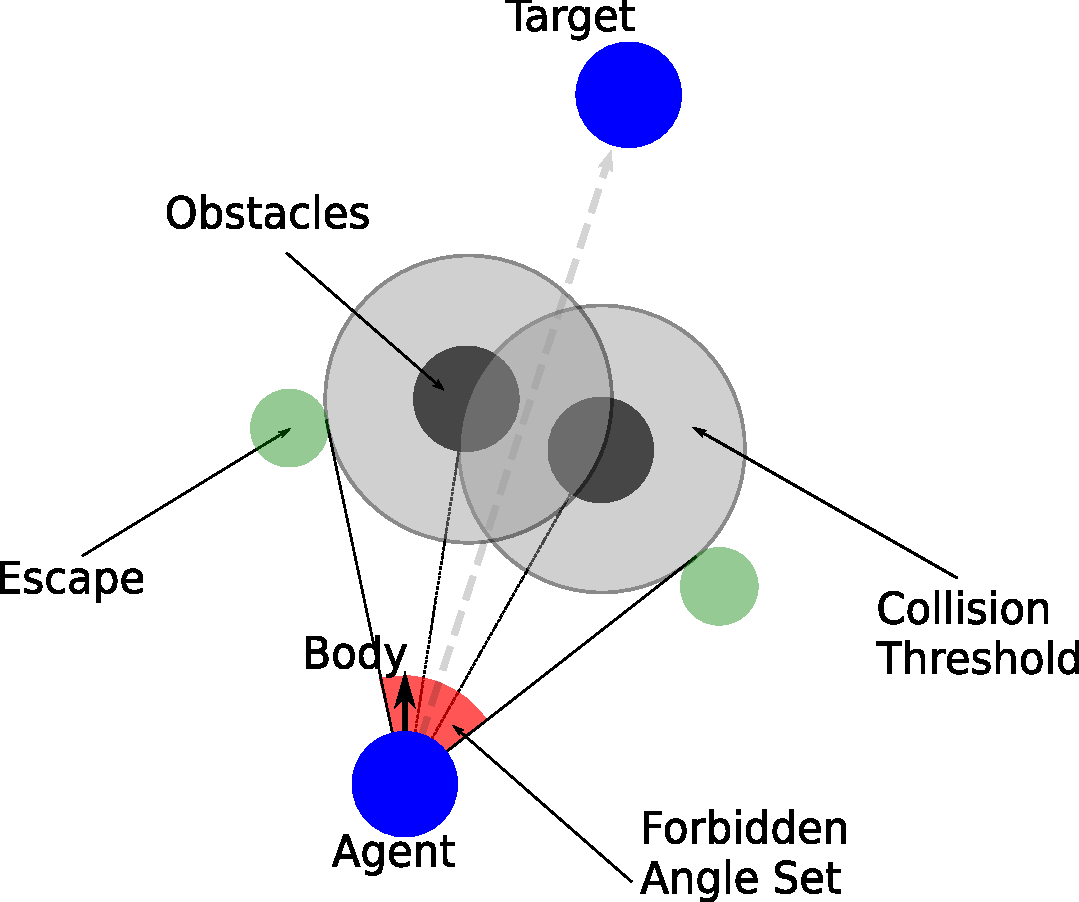
\includegraphics[width=0.3\textwidth]{figures/ObstacleAvoidance.pdf}
\end{figure}


\begin{algorithm}[H]
\caption{Escape Angle Set Calculation}
\begin{algorithmic}[1]
\begin{footnotesize}
\STATE {\bf Input: }$Obstacles = \lbrace O_{1},O_{2},...,O_{n} \rbrace $
\STATE {\bf Output: }$EscapeAngleSet$
\STATE
\FOR{$i = 1 \textbf{ to } n$}
\STATE find $LeftEscapeAngle_i$ for obstacle $O_i$
\STATE find $RightEscapeAngle_i$ for obstacle $O_i$
\ENDFOR
\STATE $EscapeAngleSet = \emptyset$
\FOR{$i = 1 \textbf{ to } n$}
\IF{$LeftEscapeAngle_i \not\in [LeftEscapeAngle_j,RightEscapeAngle_j], \forall  j\neq i$}
\STATE $EscapeAngleSet = EscapeAngleSet \cup \{LeftEscapeAngle_i\}$
\ENDIF
\IF{$RightEscapeAngle_i \not\in [LeftEscapeAngle_j,RightEscapeAngle_j], \forall  j\neq i$}
\STATE $EscapeAngleSet = EscapeAngleSet \cup \{RightEscapeAngle_i\}$
\ENDIF
\ENDFOR
\RETURN $EscapeAngleSet$
\end{footnotesize}
\end{algorithmic}
\end{algorithm}

\end{itemize}

	
	
    \item[Walk to Ball] Makes the agent walk towards the ball and stop when the ball is close enough to perform a kick.
    \begin{itemize}
    \item It performs the Turn to Ball action and then walk towards the ball, slowing down when it comes close to the ball.
    \item Ball distance returned by the vision perceptor is the distance between the camera, which is attached to agent's head, and the ball.
    \item Forward kinematics along the sagittal plane of the robot to derive the current height of the camera.
    
    	\begin{figure}[H]
\centering
  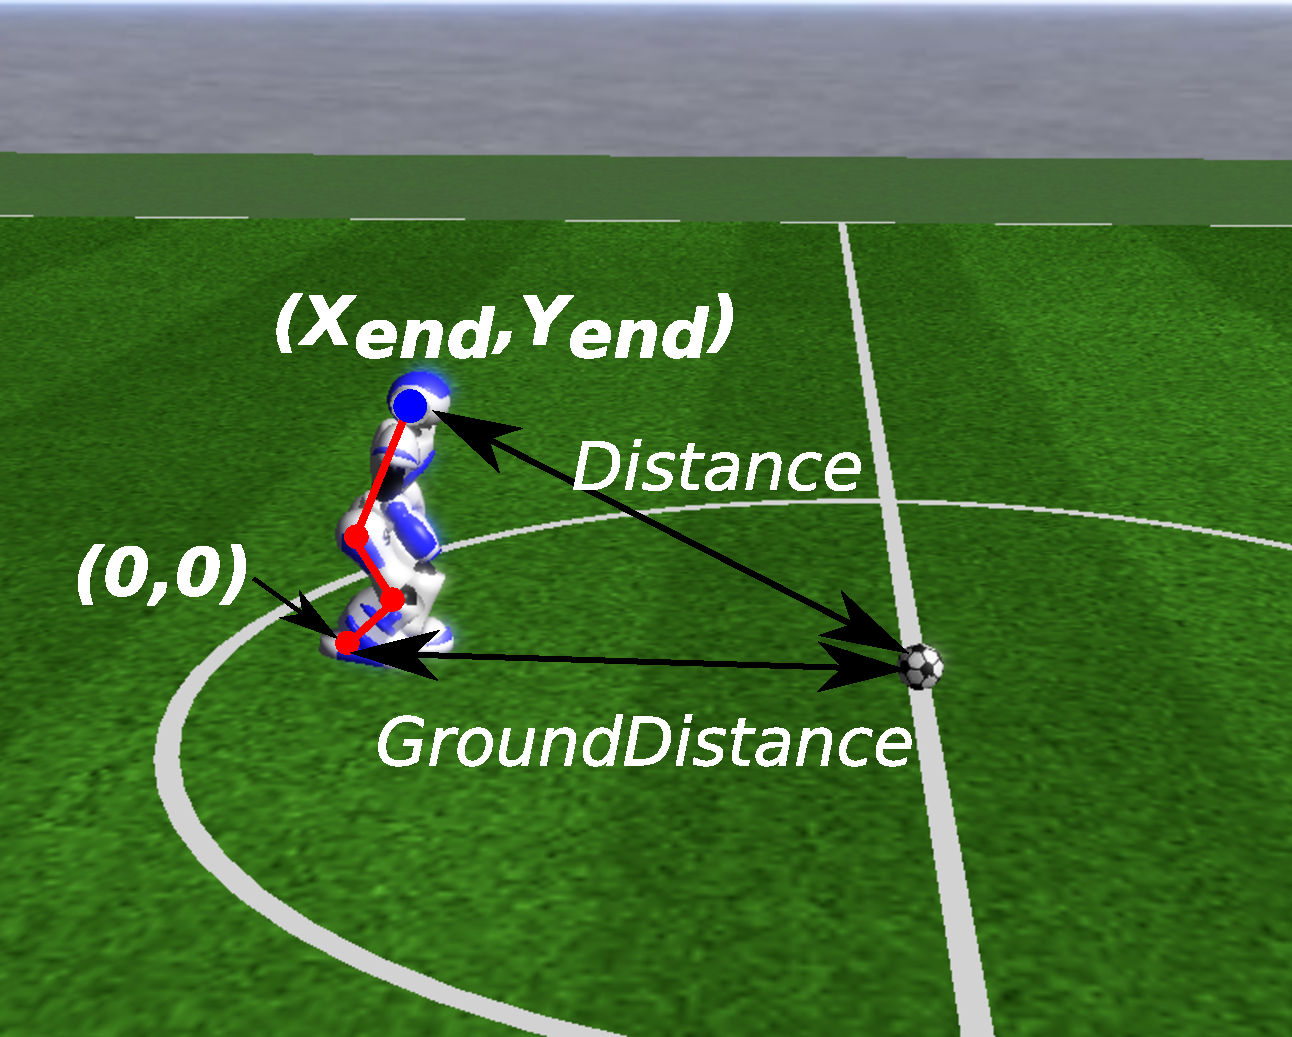
\includegraphics[trim=0cm 4cm 3cm 4cm,clip,width=0.6\textwidth]{figures/2dkinematics.pdf}
\end{figure}

	Having the ball distance and the height of the camera, the ground distance can be easily derived using the Pythagorean Theorem. 
\[
GroundDistance = \sqrt{BallDistance^2 + CameraHeight^2}
\]
	\end{itemize}	
	\item[On Ball Action] This action moves the agent close to the ball and executes an appropriate kick depending on the current state of the game.
	\begin{itemize}
	\item It first performs the Walk To Ball action in order to reach the ball.
	\item After the successful completion of the Walk To Ball action, the agent performs the Find Opponent's Goal action.
	\item Subsequently, it aligns itself with the direction of the opponent's goal.
	\item The precision of this alignment is inversely proportional to the distance from the opponent's goal.
	\item Afterwards, it performs the Position for Kick action and finally it executes a kick motion.
	\end{itemize}
    \item[Walk to Coordinate] This action moves the agent to a specific location $(x_t, y_t, \theta_t)$ in the field.\\
    \begin{align*}
\phi &= \text{atan2}(x_t-x_a,y_t-y_a)\\
d &= \sqrt{(x_t-x_a)^2 + (y_t-y_a)^2}
\end{align*}
	\begin{figure}[H]
\centering
  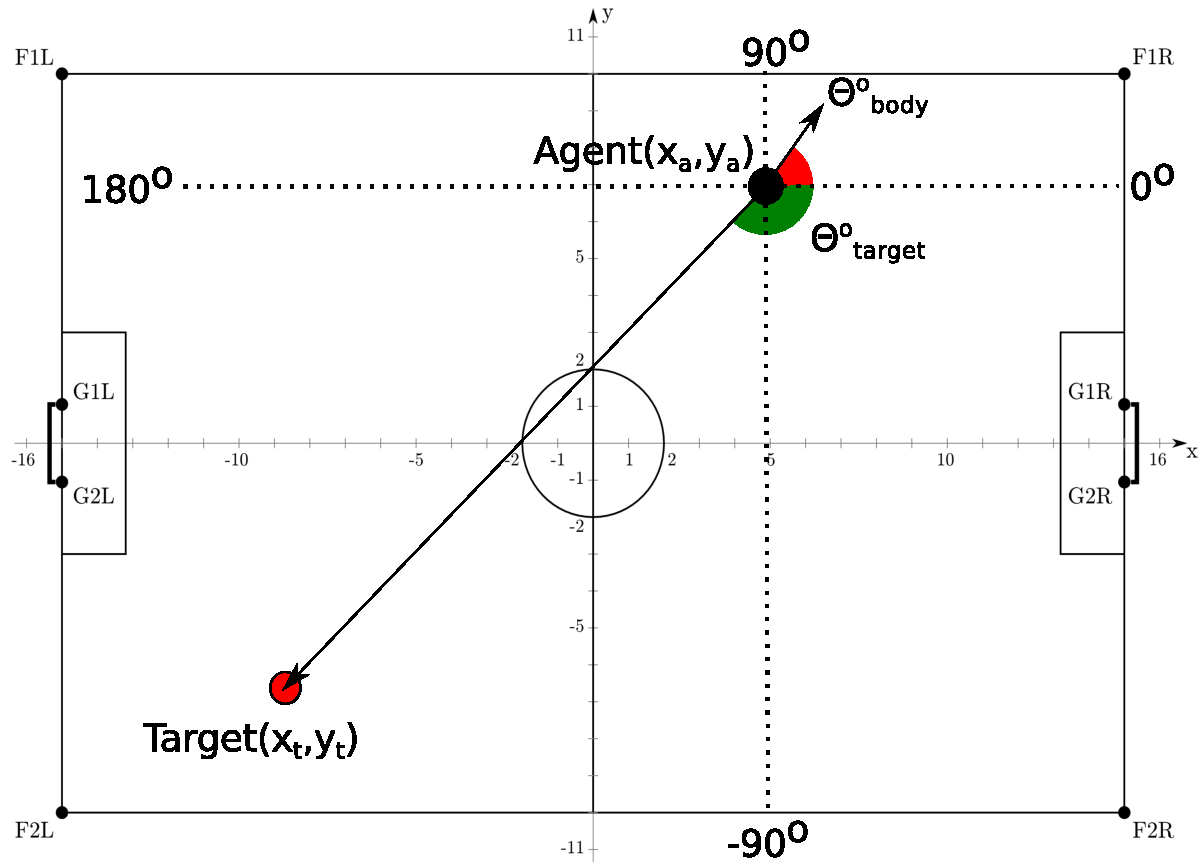
\includegraphics[width=0.4\textwidth]{figures/GoToPos.pdf}
\end{figure}
    \begin{itemize}
    \item Distance and direction are recalculated as the agent makes progress toward its target.
    \item After the position $(x_t,y_t)$ has been reached, a final rotation in place turns the agent towards the desired direction $\theta_t$.
    \item The action terminates when the agent reaches the desired location $(x_t, y_t, \theta_t)$.
    \end{itemize}
    \item[Walk To Direction] This action makes the agent walk towards a specific direction.
    \begin{itemize}
    \item It employs a turn in-place action to align with the given direction and then a straight walk action to move along the given direction.
    \item This action is not terminated by itself but there has to be a new action request.
    \end{itemize}
    \item[Dribble Ball To Direction] This action attempts to dribble the ball towards a specific direction.
    \begin{itemize}
    \item It is quite similar to the Walk To Direction action, however the agent  tries to keep the ball in front of its feet at all times. 
    \item This action is not fully functional in our software.
    \end{itemize}    
    \end{description}
   
    
  \end{frame}
  
  \subsection*{Communication}
  \begin{frame}[allowframebreaks]

    \frametitle{Communication}
    Communication in Simspark is not ideal. There are no restrictions about the use of the say effector and every agent can use it at each cycle. However, the hear perceptor comes with some restrictions.
    \begin{itemize}
    \item The agent processes are not allowed to communicate with each other directly, but the agents may exchange messages via the simulation server.
    \item Messages should not have a length of more than 20 ASCII characters.
    \item Messages shouted from beyond a maximal distance (currently 50 meters) cannot be heard.
    \item Only one message can be heard at any given time and messages from the same team can be heard only every other cycle.
    \end{itemize} 
    \newpage
	 A simple communication protocol has been created in which time is sliced into pieces lasting one server cycle (20ms) each and repeats every three cycles (60ms).
	 \begin{figure}[H]
\centering
  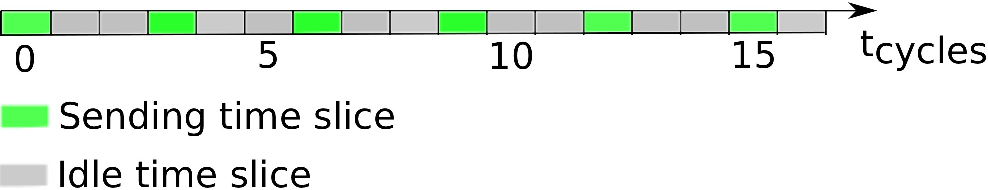
\includegraphics[width=0.6\textwidth]{figures/MAC.pdf}  
\end{figure}  
\begin{itemize}
\item Every time slice of the protocol has an associated integer label which indicates the uniform number of the player able to send its message at that slice.
\item This label starts at $1$ and grows by $1$ every time a player sends a message.
\item Every player can receive reliably the messages from all teammates every 540ms (27 cycles) for a team of 9 players or every 660ms (33 cycles) for a team of 11 players.
\end{itemize}


    
      
  \end{frame}
  
  \section{Team Coordination}
  
  \subsection*{General}
  
  \begin{frame}[allowframebreaks]
  
 	 \frametitle{Team Coordination}
 	 
 	 \begin{itemize}
 	 \item Agents miss a thinking process with which they will be able to decide about what action they should do for their team's benefit.
 	 \item Instead of each agent having its own behavior, players are depend on a centralized process called team coordination.
 	 \item Goalkeeper it the coordination's administrator who is going to execute this procedure.
 	 \item Team coordination is accomplished through communication.
 	 \end{itemize}
 	 Coordination's procedure is executed in several phases and not at once. These phases are:
	\begin{description}
	\item[Update coordination beliefs] Multiple world state beliefs from field players have to be 	combined in order to update our belief for the world state.
	\item[Split field player into groups] Field players are split into groups according to their significance to each game state. These groups are:
	\begin{itemize}
	\item Active
	\item Inactive
	\item Support
	\item Goalkeeper
	\end{itemize}
	\item[Compute positions for active players] All possible positions which are best candidates 	for assigning active players.
	\item[Assign actions for active players] Computation of the best two positions according to their cost.
	\item[Generate team's formation] Formation is generated according to ball's position into the soccer field.
	\item[Assign roles for all players] Team players are assigned roles in relation to the team's formation and their current position.
	\item[Find positions for support players] All possible team formation's positions which are best candidates for assigning support players there.
	\item[Assign actions for support players] Computation of the best mapping according to its cost.
	\end{description}
 	 
\begin{algorithm}[H]
\caption{Coordination Algorithm}
\begin{algorithmic}[1]
\begin{footnotesize}
\STATE {\bf Input: }$Coordination Messages = \lbrace M_{1},M_{2},...,M_{N-1} \rbrace, N = number of players $
\STATE {\bf Output: }$Actions = \lbrace A_{1},A_{2},...,A_{N-1} \rbrace$
\IF {$ Step = 1$ }
\STATE $B \leftarrow Update Beliefs() $
\ELSIF {$ Step = 2$ }
\STATE $S \leftarrow Coordination Splitter(B) $
\ELSIF {$ Step = 3$ } 
\STATE $A_{p} \leftarrow Active Positions(B,S) $
\ELSIF {$ Step = 4$ }
\STATE $A_{c} \leftarrow Active Coordination(A_{p},S) $
\ELSIF {$ Step = 5$ }
\STATE $ F \leftarrow TeamFormation(B) $
\STATE $ R \leftarrow Role Assignment(A_{c},B,F) $
\STATE $ S_{p} \leftarrow Support Positions(R,F,S) $
\ELSIF {$ Step = 6$ }
\STATE $ Support Coordination(R,F,S,B,A_{c},S) $
\ENDIF
\end{footnotesize}
\end{algorithmic}
\end{algorithm}
 	 

  \end{frame}  
  
  \subsection*{Messages and Communication}

  \begin{frame}[allowframebreaks]

    \frametitle{Messaging}
    
    Types of messages:
    \begin{description}
\item[Init Message] This type of message declares the initialization for each agent into the field. 

\begin{description}
  \item[{\bf Message format:}] 
  \texttt{i,<Uniform number> }
\end{description}

\item[Start Message] This type of message is only sent by the administrator, it declares that all agents are now initialized in the process.

\begin{description}
  \item[{\bf Message format:}] 
  \texttt{s,<Uniform number>}
\end{description}
\newpage

\item[Coordination Message] This is the most important type of message. It includes information about each agent's beliefs. There are four types of these messages in respect to the agent's situation in the game. these types are:
\begin{description}

\item[Type C] Agent has complete awareness of the world state. He sends his uniform number, his position and the ball's position accurately.

\begin{description}
  \item[{\bf Message format:}]
  \texttt{c,<Uniform number>,<Agent X>,<Agent Y>,<Ball X>,<Ball Y>}
\end{description}

\item[Type L] Agent has complete awareness only for his position in the field, ball is not in his field of view.
\begin{description}
  \item[{\bf Message format:}]
  \texttt{ l,<Uniform number>,<Agent X>,<Agent Y>}
\end{description}

\item[Type B] Agent has complete awareness only about the ball's distance from his body, its horizontal, and its latitudal angle.

\begin{description}
  \item[{\bf Message format:}] 
  \texttt{b,<Uniform number>,<Ball Distance>,<Ball Horizontal-Angle>}
\end{description}

\item[Type X] Agent has complete unawareness of the world state.

\begin{description}
 \item[{\bf Message format:}]
 \texttt{x,<Uniform number>}
\end{description}

\newpage

\end{description}
\item[End Message]
This type of message serves to stop field players from sending coordination messages.
\begin{description}
  \item[{\bf Message format:}] 
  \texttt{e,<Uniform number>}
\end{description}
\item[Action Message]
These messages are only sent by the administrator in the end of the coordination procedure, when actions for all field players have been computed.
\begin{description}
  \item[{\bf Message format:}]
  \texttt{a,<Uniform number>,<Action ID>,<Action parameter 1>,
  <Action parameter 2>,<Action parameter 3>}
\end{description}
\end{description}
\newpage

Messaging Process:
\begin{itemize}
\item Agents have to initialize their presentation into the field with ``init'' messages.
\item Goalkeeper saves these messages in a temporal array and when this array implies that all field players have been initialized themselves, sends them a ``start'' message.
\item Field players send ``coordination'' messages to the goalkeeper.
\item When goalkeeper gathers these messages from all field players, sends them an ``end'' message to stop them from broadcasting unnecessarily.
\item The next phase of this process is the execution of the coordination algorithm which lasts for six simulation cycles, approximately 120ms.
\item When coordination's administrator is ready to broadcast computed actions to field players, goalkeeper uses ``action'' messages in order to accomplish this procedure.
\item After this phase, the same process is repeated after a timeout which can be defined manually.
\end{itemize}

\begin{figure}[H]
\centering
  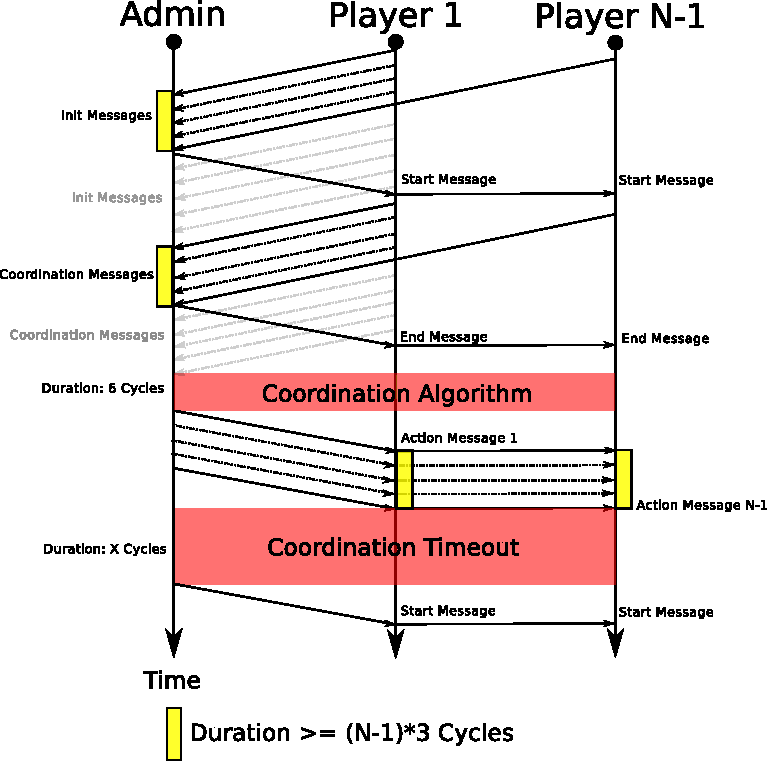
\includegraphics[width=0.6\textwidth]{figures/CoordComm.pdf}
\end{figure}

   
  \end{frame}

  \subsection*{Coordination's Beliefs}

  \begin{frame}
    \frametitle{Coordination's Beliefs}
    
    \begin{quote}
    How could a specific agent, in a multi-agent environment, have the adequate knowledge about the state of the world, receiving different observations from different agents?
    \end{quote}
    
    This agent has to combine all these observations, without knowing which of them are faulty or correct, in order to obtain a realistic representation of the world.\\
    
    \textbf{What do we need to know?}
        
   
    \begin{itemize}
    \item Ball position
    \item Agents positions
    \item Agents distances from ball
    \end{itemize}

  \end{frame}
  
  \begin{frame}[allowframebreaks]
    \frametitle{Ball Position}
    Observations source:
    \begin{itemize}
    \item Agents who have sent ``type C'' coordination messages.
    \item Goalkeeper uses his own observation too.
    \end{itemize}
    Weighted Observation Sets:
    \begin{align*}
	{\bf Obsevation_{i} } &= (x,y) \\ 
	{\bf Weight_{i}} &= 1
	\end{align*}
	
	These observations sets are correlated, for every two sets which are been correlated, a new set is formed which contains observations from the two parent sets. The weight of the new set will be the sum of its parents' weight.
	
	\newpage
	
	\begin{align*}
{\bf Obsevation Set_{i} } &= \lbrace (x_{1},y_{1}),...,(x_{k},y_{k}) \rbrace \vee k \in [1,n] , k\in \mathbb{Z} \\
{\bf Weight_{i}} &= k
\end{align*}

Consequently, we have to compute our belief about ball position.
Given a total number of N-observations, n-observation's sets, each one of them has k-observations, the final ball belief will be:\\
\begin{align*}
{\bf Ball Belief} = \displaystyle\sum\limits_{i=1}^n \frac {Weight_{i}} {N \ast k}  \displaystyle\sum\limits_{j=1}^k Obsevation Set_{i}[j]
\end{align*}
    
 
  \end{frame}
  
  
	\begin{frame}
    \frametitle{Agents' distance from ball}
    \begin{itemize}
    \item For agents who have sent ``Type C'' and ``Type L'' coordination messages and they are able to know their exact position in the field, this distance is calculated by finding the distance between the ball belief's position and the agent's position.
    \item For agents who have sent ``Type B'' coordination messages we just take the distance part of the message.
    \item For agents who have sent ``Type X'' messages we assume $\infty$ distance.
    \end{itemize}   
    \end{frame}  
  
  
  \subsection*{Subsets into Coordination}
\begin{frame}

    \frametitle{Subsets}
    
    \begin{itemize}
    \item The existence of multiple agents makes coordination function be too complex and computationally expensive to solve.
    \item Split players into subsets would make easier for us to coordinate their actions in real-time.
    \end{itemize}
    there are three subsets:
    \begin{description}
    \item[Active] Active subset consists of three agents and it is the most important set of agents in the coordination.
    \item[Support] Support subset consists of agents who are neither in the active subset nor in the inactive one.
    \item[Inactive]Inactive subset consists of agents who have sent ``Type X'' messages. Agents who constitute this subset assigned the same action, to find their positions in the field.
    \item[Goalkeeper] Agent with the uniform number one is selected to be this agent which is responsible for guarding our goal.
    \end{description}
 
 \end{frame}  
  
  
  \begin{frame}[allowframebreaks]

    \frametitle{Coordination Splitter}
    \begin{quote}
    How the above three groups are generated by coordination splitter?
    \end{quote}
    \begin{itemize}
    \item An array full of team's agents is sorted according to the distance each agent has from the ball.
    \item We assign to the active subset the agents in the three first positions of the sorted array.
    \item Other agents with distance less than infinity join the support subset.
    \end{itemize}
    
    \newpage
    
    \begin{figure}[H]
	\centering
  	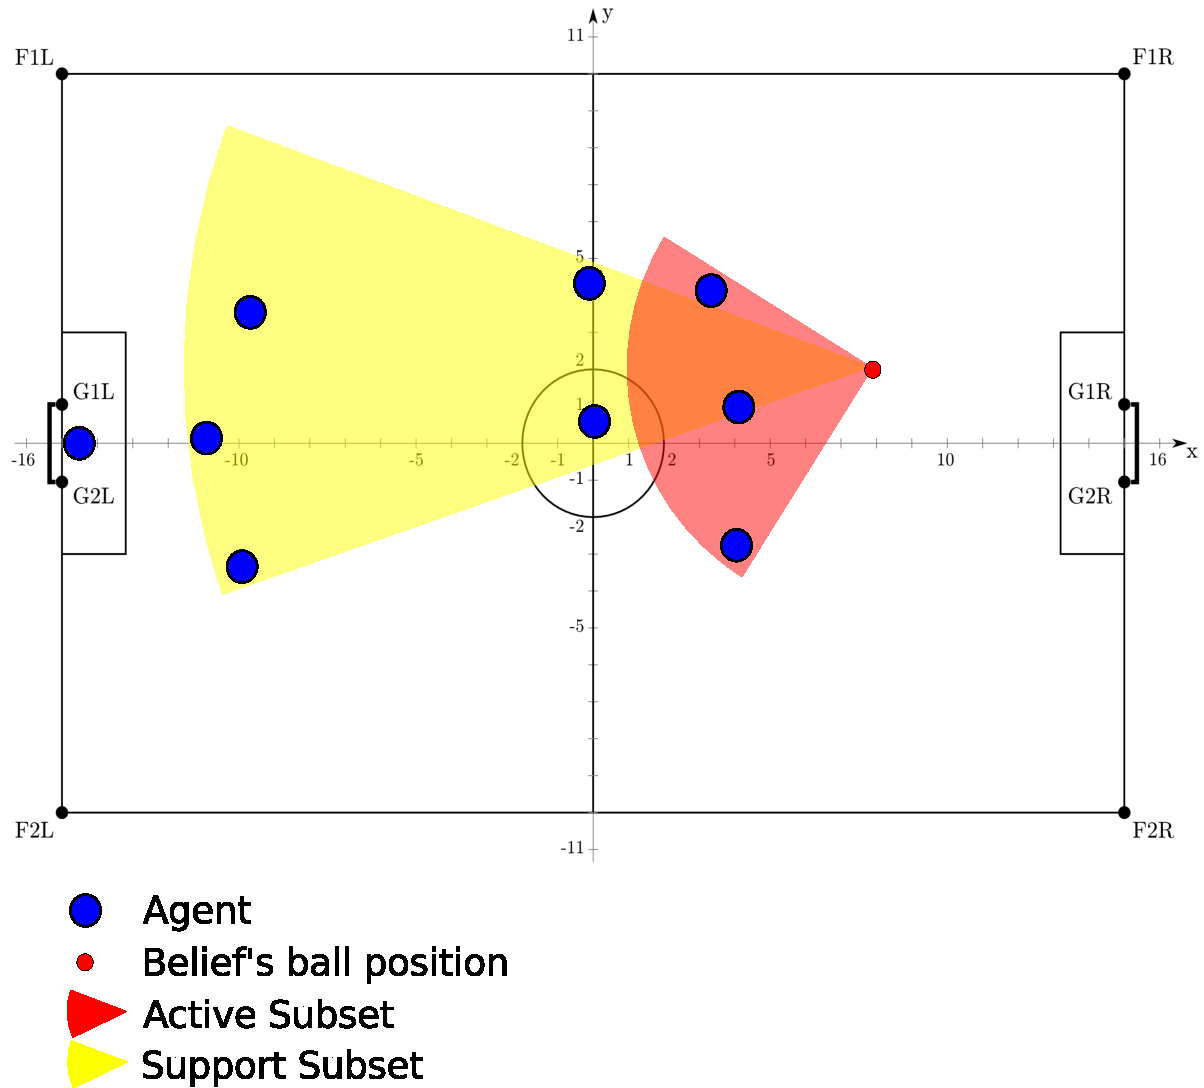
\includegraphics[width=0.6\textwidth]{figures/Splitter.pdf}
	\end{figure}
  
  \end{frame} 
  
  \subsection*{Soccer Field Value}
  \frame
  {
    \frametitle{Soccer Field Value}
    
    \begin{figure}[H]
	\centering
  	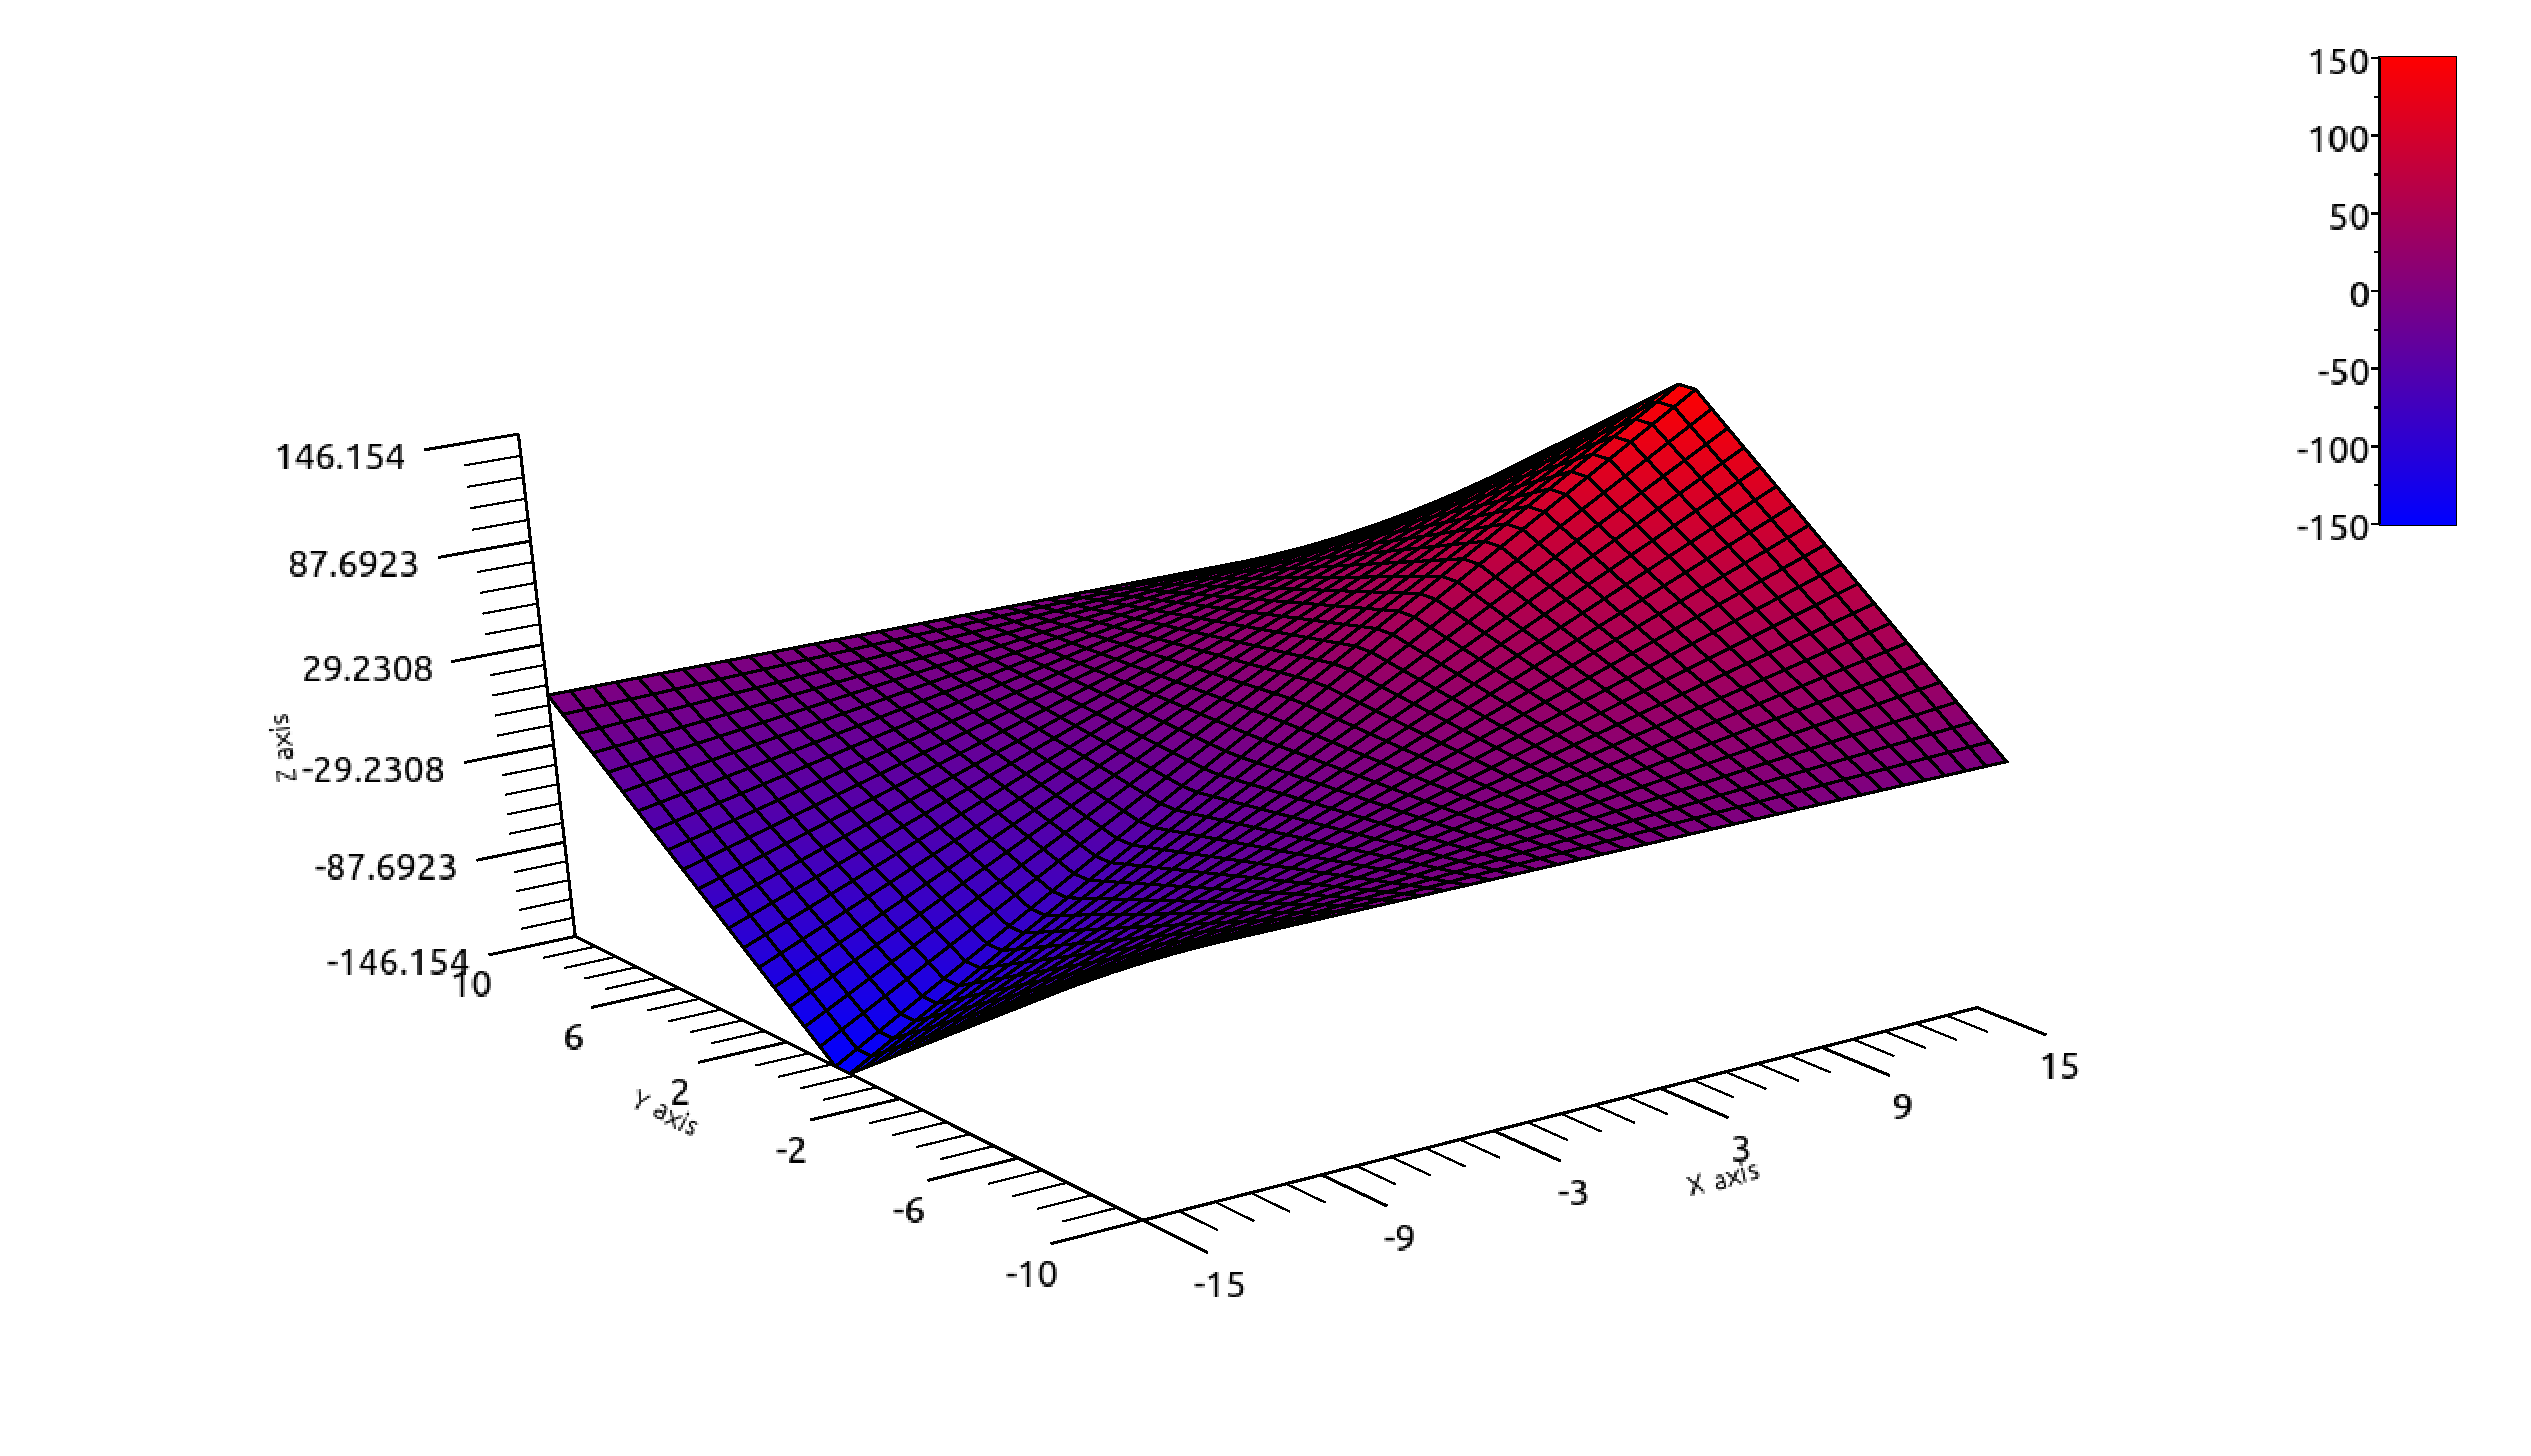
\includegraphics[width=\textwidth]{figures/Graph1.pdf}

	\end{figure}
 
  }
  
  
  \subsection*{Active Coordination}
  
  
 \frame
  {
    \frametitle{On Ball Player}
    
    An agent from the active subset has to be selected to do an action related to the ball. We have to find the agent who has minimum cost according to two parameters:
	\begin{enumerate}
	\item \textbf{Distance from ball} $d_{i}$ 
	\item \textbf{Angle towards goal} $\vartheta_{i}$
	\end{enumerate}
	Given an active subset:
	\begin{align*}\
	{\bf ActiveSubset} &= \lbrace Agent_{1},Agent_{2},Agent_{3} \rbrace  \\
	{\bf Cost_{i}} &= d_{i} + a \times \vartheta_{i}, a\in\mathbb{R} \\
	{\bf OnBallPlayer} &= \arg\min_{i}(Cost_{i})
	\end{align*}
	Additionally, we give to the agent who had been assigned an action towards the ball in the previous coordination cycle a small advantage over the others to be again the on ball player.
 
  }  
  
  
  
  \begin{frame}[allowframebreaks]
    \frametitle{Active Positions}
    Possible candidate positions for the rest players who are assigned to the active subset.
    \begin{itemize}
    \item Depend on the position of the ball.
    \item Defensive or offensive approach to compute these positions.
    \item In both cases we create an array of equidistant coordinates which are located in a radius which is determined by the ball's location and they are not out of soccer field's limits.
    \item From these candidate positions we keep only a max number of nine positions according to their values.
    \end{itemize}
    
    \newpage
    
    \begin{figure}[H]
	\centering
	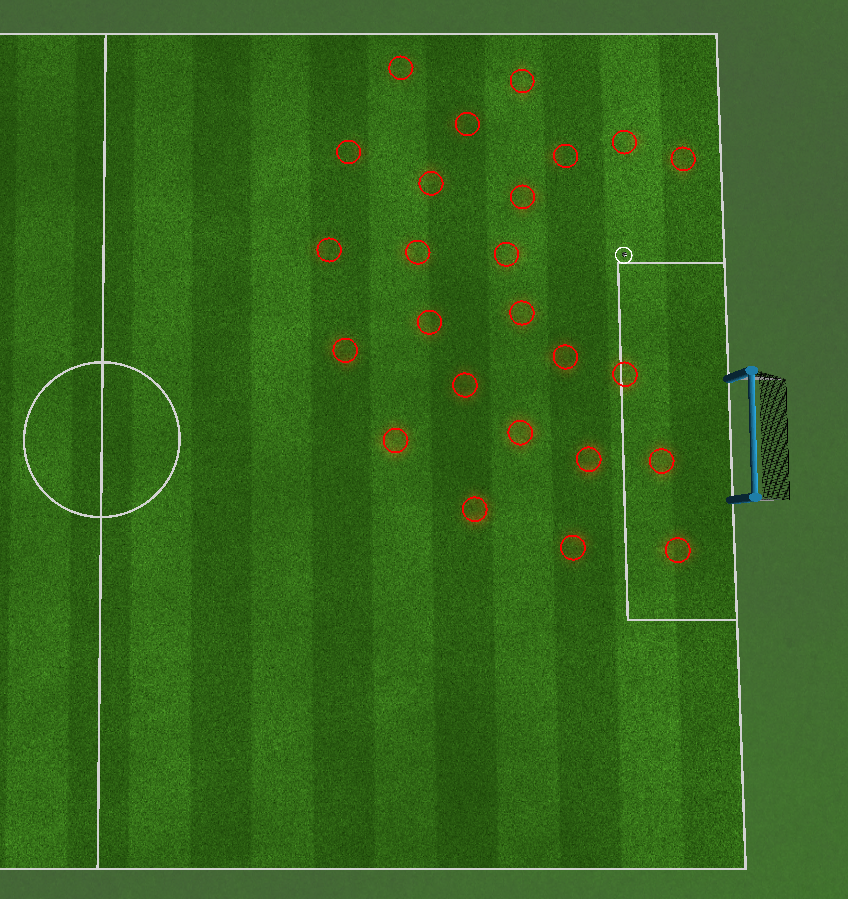
\includegraphics[height=5cm]{figures/ActivePositions2.png}\		
  	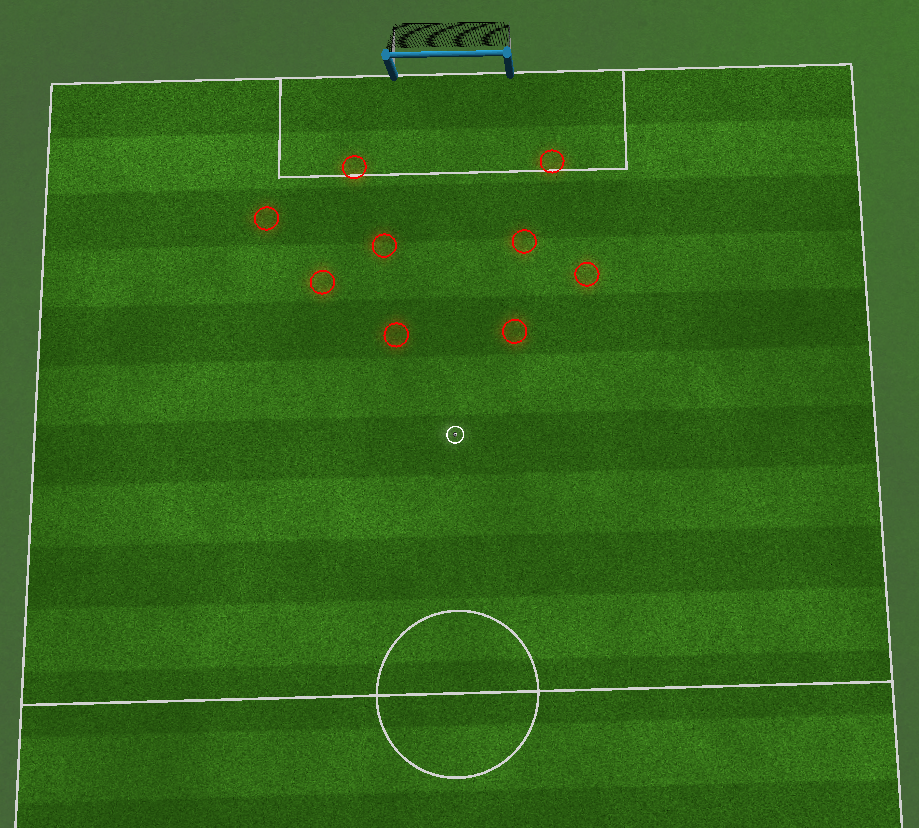
\includegraphics[height=5cm]{figures/Active3.png}
	\end{figure}
 
  \end{frame}
  
 \frame
  {
    \frametitle{Active Mapping}
    \begin{itemize}
    \item 2 Players
    \item 9 Positions
    \end{itemize}
    We have to find which positions from these nine can be assigned to the two agents with the minimum cost. Making use of a brute force algorithm we compute the cost for each and every combination of possible mappings. Using a brute force method the number of possible mapping remains able to be computed in real-time. Assuming maximum number of active positions in our case nine, the possible mappings are: ${{9}\choose{2}} = 72$ mappings.
 
  }  
  
  \begin{frame}[allowframebreaks]
  \frametitle{Properties for Active Mapping}
  

	\begin{enumerate}
	\item \textbf{Total distance }$C_{d}$ - Total distance agents have to travel in order to reach in their optimized mapping positions.
	\item \textbf{Possible Collisions }$C_{c}$ - In each mapping we check every combination of two agents and their assigned positions if it is possible for them to collide with each other.
	\item \textbf{Field's value }$C_{v}$ - Agents will try to maximize this cost according to the game's state and the value which has every position in the field.
	\item \textbf{Close routes }$C_{r}$ - Agents routes should be safe, so we calculate the difference between start positions' distance and target positions' distance.
	\item \textbf{Neighboring positions }$C_{p}$ - In general agents will try to avoid be assigned in neighboring positions. So if their target positions are near to each other this is going to add more cost.
	\item \textbf{Positions aligned to X-axis }$C_{a}$ - We want team stretching into the field in order to have players in most regions of the soccer pitch.
	\end{enumerate}
	\begin{align*}
	Total cost &= C_{d,i}+C_{c,i}-C_{v,i}-C_{r,i}-C_{p,i}-C_{a,i}\\
Optimized Cost &= \arg\min_{i}(TotalCost_{i})
	\end{align*}
  
  
  \end{frame}
 
 \subsection*{Team Formation}
  
  \frame
  {
    \frametitle{Team Formation 9-Players Version}
    \begin{figure}[t!]
	\centering
 	 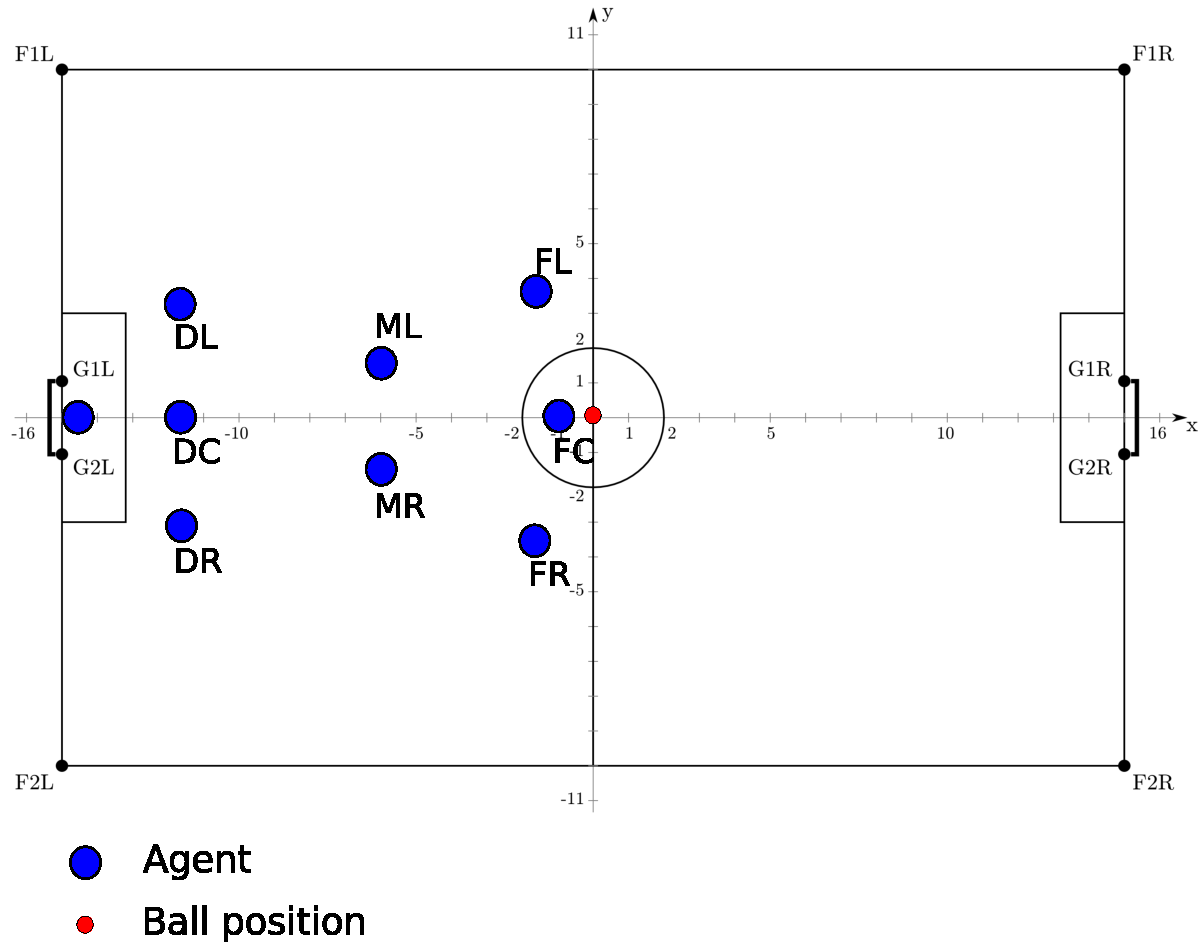
\includegraphics[width=0.7\textwidth]{figures/Formation9_0.pdf}
	\end{figure}
 
  }
  
  \frame
  {
    \frametitle{Team Formation 11-Players Version}
    \begin{figure}[H]
	\centering
 	 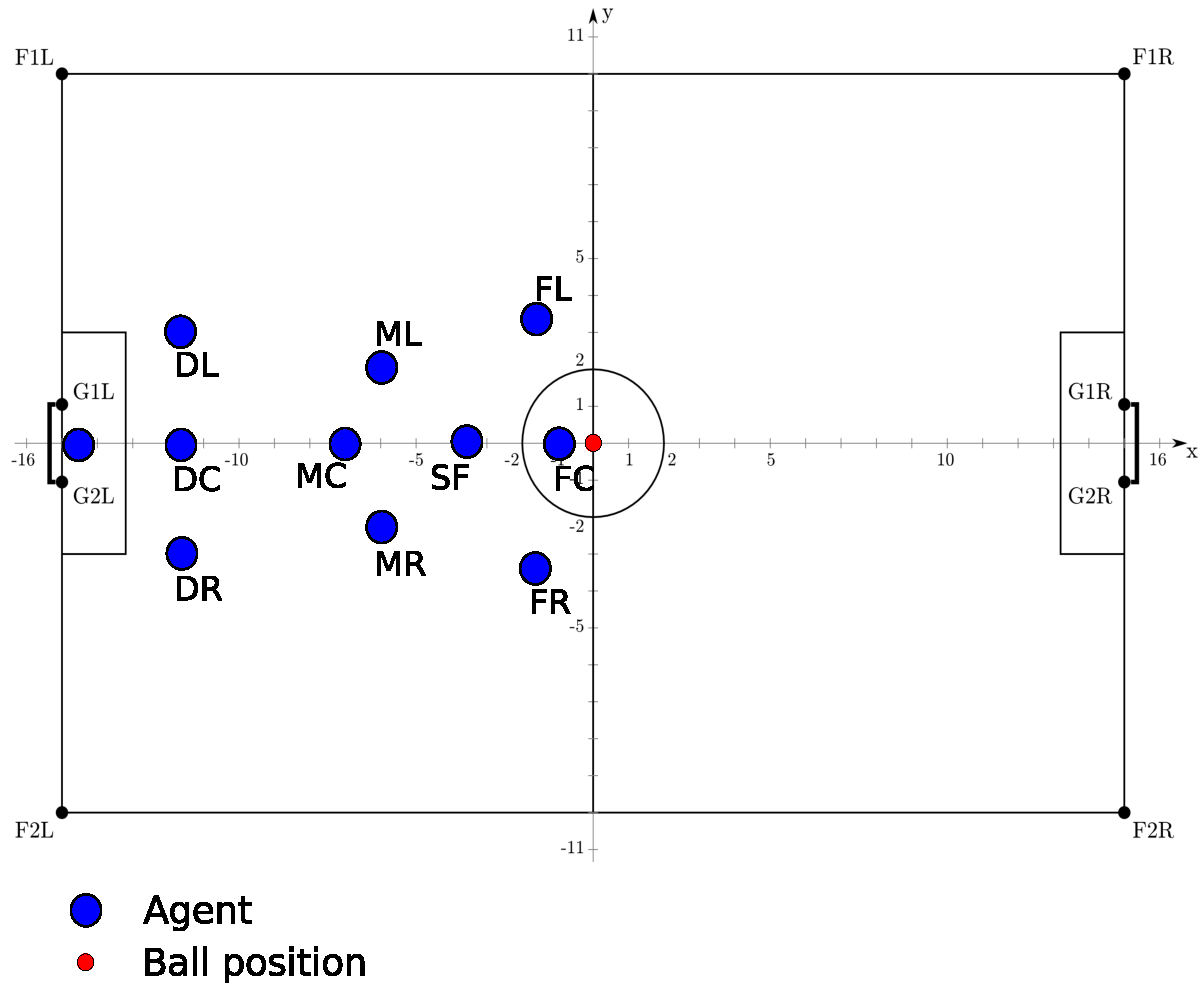
\includegraphics[width=0.7\textwidth]{figures/Formation11_0.pdf}
	s\end{figure}
 
  }
  
  \subsection*{Role Assignment}
  	\begin{frame}[allowframebreaks]
    \frametitle{Role Assignment}
    
    Given a computed team formation we have to assign roles to the active subset's players.
    
    \begin{itemize}
    \item So, for N active players we choose N team formation positions which minimize the distance from the ball.
    \item Roles which these positions represent will be assigned to the active players.
    \end{itemize}
        
    \newpage
    
    \begin{figure}[t!]
	\centering
  	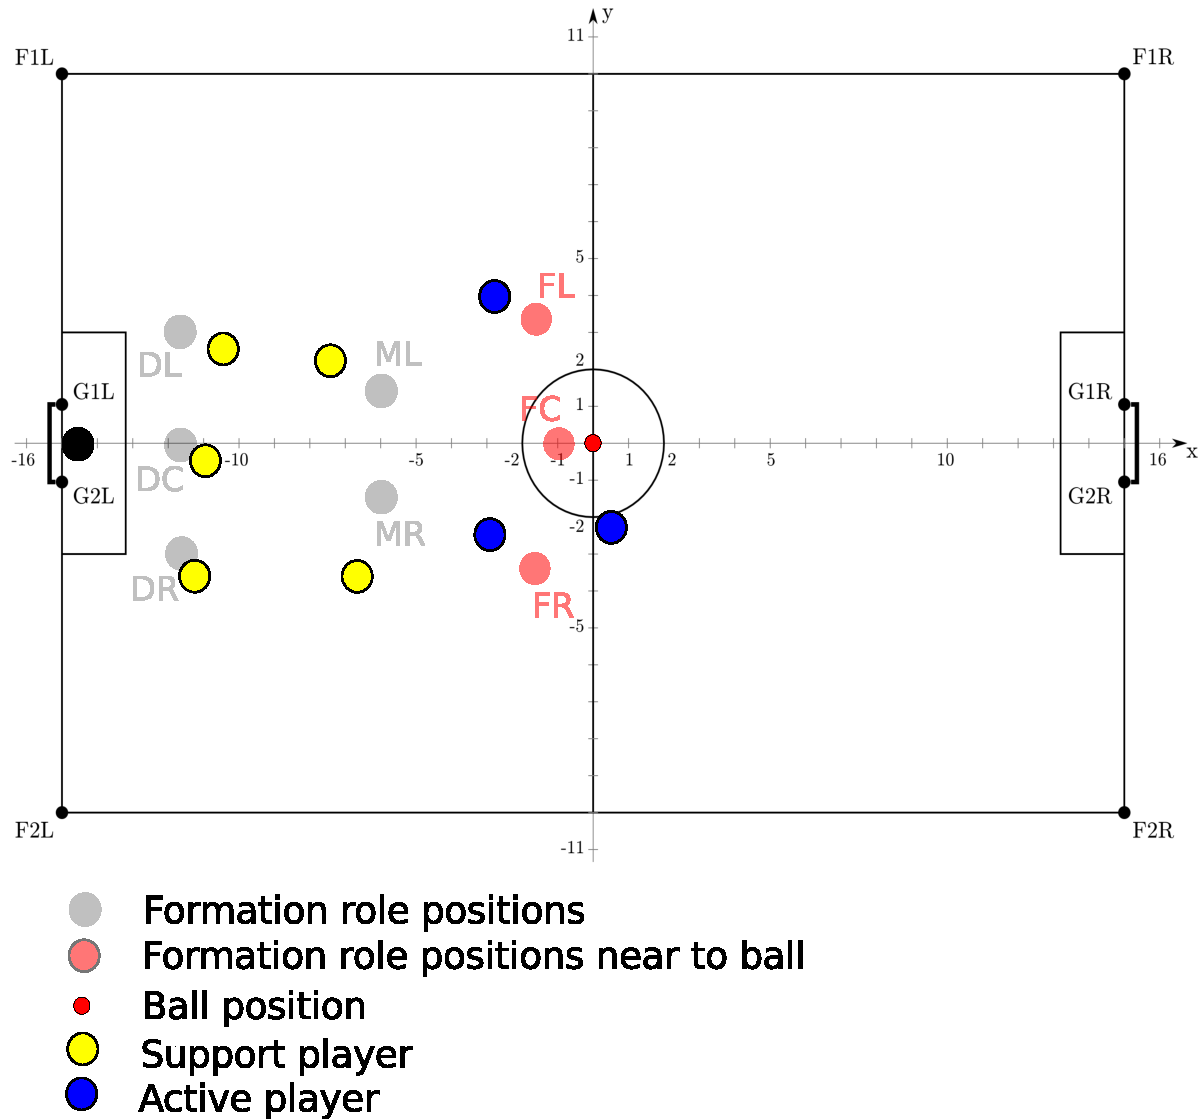
\includegraphics[width=0.7\textwidth]{figures/RoleAss.pdf}
	\end{figure}

  	\newpage
  
	\begin{figure}[H]
	\centering
  	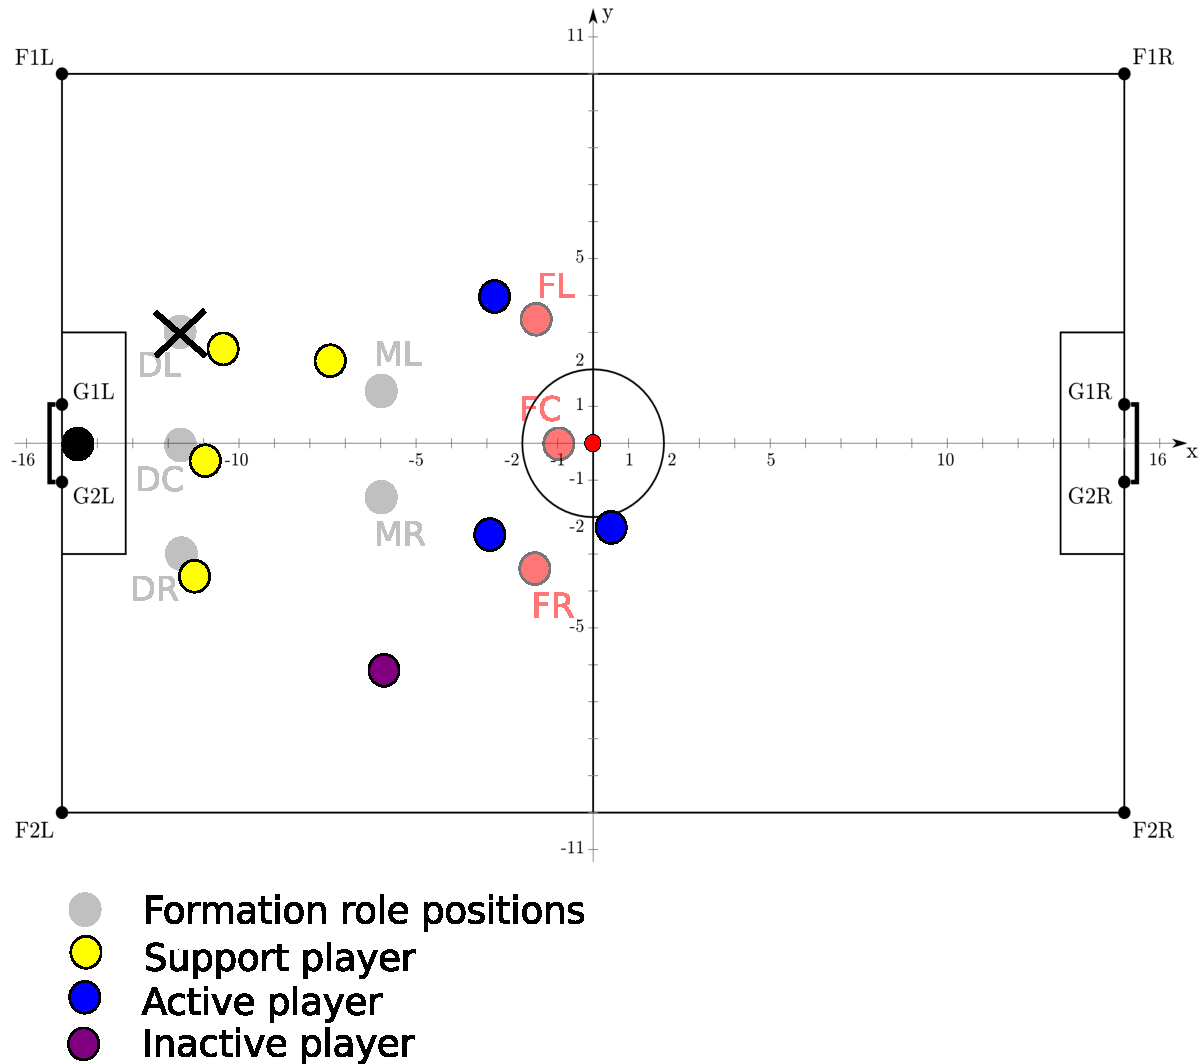
\includegraphics[width=0.7\textwidth]{figures/SupportPos.pdf}
	\end{figure}
  
  	\end{frame}

  	\subsection*{Support Coordination}
  
 	\begin{frame}[allowframebreaks]
  
 	 \frametitle{Support Coordination}
  
  	\begin{itemize}
  	\item Same number from positions, agents.
  	\item Brute force algorithm for 9 players, factorial complexity, $\leqslant 5! \Leftrightarrow  	{{5}\choose{5}} = 120$ mappings. 
 	 \item For 11 players, factorial complexity,$ 7! \Leftrightarrow  {{7}\choose{7}} = 5040$ mappings. 
  	\end{itemize}
	\begin{quote}
	Solution?
	\end{quote}
  	\textbf{Dynamic programming algorithm}, based on a simple property.
	\begin{theorem}
	For every mapping there is a subset of a lower cost with which we can reduce the cost of the complete mapping by augmenting it with that of the subset's lower cost mapping.
	\end{theorem}  
	
	\newpage
	
	\begin{algorithm}[H]
\caption{Dynamic programming implementation}
\begin{algorithmic}[1]
\begin{footnotesize}
\STATE {\bf Input: }$SupportPlayers = \lbrace A_{1},A_{2},...,A_{n} \rbrace$
\STATE {\bf Input: }$SupportPositions = \lbrace P_{1},P_{2},...,P_{n} \rbrace $
\STATE {\bf Output: }$OptSupportMap$
\STATE $OptSupportMap = \varnothing $
\FOR{$k = 1 \to n$} 
\FOR{{\bf each} $\alpha$ in SupportPlayers}
\STATE $ S = {{n-1}\choose{k-1}} $, sets of k-1 agents for supportPlayers - $\lbrace \alpha \rbrace$
\FOR{{\bf each} s in S}
\STATE $SupportRoleMap$ $m_{0}$ = $RoleMap[s]$
\STATE $SupportRoleMap$ $m$ = $m_{0}$ $ \cup (\alpha \rightarrow P_{k})$
\STATE $OptSupportMap[\lbrace \alpha \rbrace \cup s] = mincost(m,OptSupportMap[\lbrace \alpha \rbrace \cup s])$
\ENDFOR
\ENDFOR
\ENDFOR
\end{footnotesize}
\end{algorithmic}
\end{algorithm} 

	As we see in this table, an optimal mapping is built iteratively for position sets from $\lbrace P_{1} \rbrace$ to $\lbrace P_{1},P_{2},...,P_{n} \rbrace$. In every step of this algorithm we use the lower cost's mapping for a subset of agents and positions which are compatible with our current mapping.

	\begin{table}[t!]
	\label{tab:DynamicTable}
	\centering
	\begin{small}

    \begin{tabular}{ | c | c | c | }
    \hline
    $\lbrace P_{1} \rbrace$   & $\lbrace P_{1},P_{2} \rbrace$ 	& $\lbrace P_{1},P_{2},P_{3} \rbrace$\\ \hline
    $A_{1} \rightarrow P_{1}$ & $A_{1} \rightarrow P_{2},min(A_{2} \rightarrow P_{1})$	 	& $A_{1} \rightarrow P_{3},min(\lbrace A_{2},A_{3} \rbrace \rightarrow \lbrace P_{1},P_{2} \rbrace)$  \\ \hline
    $A_{2} \rightarrow P_{1}$ & $A_{1} \rightarrow P_{1},min(A_{3} \rightarrow P_{1})$	 	& $A_{2} \rightarrow P_{3},min(\lbrace A_{1},A_{3} \rbrace \rightarrow \lbrace P_{1},P_{2} \rbrace)$  \\ \hline
     						  & $A_{2} \rightarrow P_{2},min(A_{1} \rightarrow P_{1})$ 		& 	$A_{3} \rightarrow P_{3},min(\lbrace A_{1},A_{2} \rbrace \rightarrow \lbrace P_{1},P_{2} \rbrace)$  \\ \hline
       						  & $A_{2} \rightarrow P_{2},min(A_{3} \rightarrow P_{1})$ 		&   \\ \hline
       						  & $A_{3} \rightarrow P_{2},min(A_{1} \rightarrow P_{1})$ 		&   		\\ \hline
    						  & $A_{3} \rightarrow P_{2},min(A_{2} \rightarrow P_{1})$		&   \\
    \hline

    \end{tabular}
    \end{small}
     
	\end{table}

	\newpage

	These assignments result in a total of $ {{n-1}\choose{k-1}} $ mappings to be evaluated in each iteration. Summing to $\sum\limits_{i=1}^N{{n-1}\choose{k-1}}$ possible mappings.\\
\[
\sum\limits_{i=1}^N{{n}\choose{k-1}} = \sum\limits_{i=0}^{n-1}{{n-1}\choose{k}} = 2^{n-1}
\]

	\begin{itemize}
	\item For nine players in each team, this algorithm would not have any impact. As the previous brute force algorithm was having 5! (120 mappings), which is not much bigger computational complexity than this approach $5 \ast 2^{4}$ (80 mappings).

	\item For seven players in our support subset, this approach gives us great improvement in our coordination time, $7 \ast 2^{6}$ (448 mappings) $\ll$ 7! (5040 mappings) in comparison to the brute force algorithm.
	\end{itemize}

  
  \end{frame}
  
  
  
  
  
  \frame 
  {
    \frametitle{Properties for Support Mapping}
    \begin{enumerate}
	\item \textbf{Total distance }$C_{d}$ - Total distance agents have to travel in order to reach in their optimized mapping positions.
	\item \textbf{Possible Collisions }$C_{c}$ - In each mapping we check every combination of two agents and their assigned positions if it is possible for them to collide with each other.
	\end{enumerate}
	\begin{align*}
	Total cost &= C_{d,i}+C_{c,i}\\
Optimized Cost &= \arg\min_{i}(TotalCost_{i})
	\end{align*}
    
  
 
  }
  
  \section{Results}
  
  \subsection*{Movement}

  \frame
  {
    \frametitle{Movement Results and Improvements}
    \begin{table}
\begin{center}
\begin{footnotesize}
\begin{tabular}{ccccc}
\textbf{Motion Version} & \textbf{Walk(m/s)}	& \textbf{Turn(d/s)}	& \textbf{Kick(m)}&\textbf{Strong Kick(m)} \\  \hline
Webots (Text-Based) 		& 0.11 				& 21 				& 3 				& - \\
FIIT (XML)				& 0.22 				& 25 				& 3 (4 sec) 		& 4 (5 sec) \\
\textbf{AST\_3D} 		& 0.45 	& 30 		& 3 (2.5 sec)& 5.5 (2.5 sec) \\
\end{tabular}
\end{footnotesize}
\end{center}
\end{table}

  }
  
  \subsection*{Communication}
  
  \frame
  {
    \frametitle{Communication Results}
    \begin{table}[h!]
\begin{center}
    \begin{tabular}{ccc}
    \textbf{Communication Phase} 	& \textbf{Ideal (Cycles)}			& \textbf{During Match (Cycles)} \\
    \hline
    Init Messages 					& 24  ( 0.48 Sec ) 			& 24 	( 0.48 Sec )		\\
    Coordination Messages			& 24  ( 0.48 Sec )			& 42.5  ( 0.85 Sec )		\\
    Action Messages 				    & 24  ( 0.48 Sec )			& 24 ( 0.48 Sec )	 		\\
    \end{tabular}
\end{center}
\end{table}

  }


  \subsection*{Coordination}
  \frame
  {
    \frametitle{Coordination Results}

  }

  \subsection*{GoalKeeper}
  \frame
  {
    \frametitle{Goalkeeper Results}
    
    \begin{table}[h!]
\begin{center}
    \begin{tabular}{cc}
    \textbf{GoalKeeper Type} 	& \textbf{Goals Conceded}\\
    \hline
    No Goalkeeper						& 7\\
    Goalkeeper with ``Empty'' Behavior	& 7\\
    Goalkeeper with ``Full'' Behavior	& 3\\
    \end{tabular}
\end{center}
\end{table}
    
    

  }
  
  \subsection*{Games}
  \frame
  {
    \frametitle{Full-Games Results}
    
 \begin{table}[h]
\begin{center}
    \begin{tabular}{cccccc}
    \textbf{Team} 	& \textbf{W} & \textbf{D} & \textbf{L} & \textbf{AGD} & \textbf{Games}   \\
    \hline
    UTAustinVilla 	& 0		& 0		& 4		& -5.2		& 4 			\\
    Robocanes 		& 0		& 0		& 1		& -6.0		& 1 			\\
    BeeStanbul		& 0		& 0		& 3		& -4.0		& 3				\\
    NomoFC 			& 1		& 2		& 0		& +0.3 		& 3 			\\
    Rail 			& 0		& 4		& 0		& 0.0 		& 4 			\\
    OxBlue 			& 0		& 0		& 2		& -1.5 		& 2 			\\
    FUTK3D 			& 0		& 5		& 0		& 0.0 		& 5 			\\
    FARZANEGAN 		& 1		& 1		& 0		& +0.5 		& 2 			\\
    MAK 			    & 2		& 0		& 0		& +2.0 		& 2 			\\
    L3M-SIM			& 3		& 2   	& 0		& +0.6 		& 5 			\\     
    \end{tabular}
\end{center}
\end{table}
    
    

  }

  \section{Conclusion}

  \frame
  {
    \frametitle{Future Work}
Reaching to a level to oppose teams that have already participated in this robotic soccer competition gives us an incentive to keep working in order to improve further our team. In this section, we present some of these possible improvements.  
\begin{itemize}
\item Probabilistic Localization System
\item Dynamic Omni-Directional Movement
\item Passing
\item Testing and Debugging in New Server's version
\item Participation in Robocup
\end{itemize}


  }

  \frame
  {
    \frametitle{Final}
    

  }


\end{document}
